% =============================================================================
% InnoBeweegLab — Background Research Report
% Main file: assembles the title page, front matter, and each chapter file
% from sections/*.tex. Compile with: latexmk -pdf main.tex
% =============================================================================
\documentclass[11pt,a4paper]{article}

% ---------- encoding / fonts ----------
\usepackage[utf8]{inputenc}
\usepackage[english]{babel}
\sloppy
\tolerance=2000
\emergencystretch=2em

% ---------- page geometry ----------
\usepackage[margin=2.5cm]{geometry}
\usepackage[hyphens]{url}

% ---------- color palette (matches the project's Word house style) ----------
\usepackage{xcolor}
\definecolor{navy}{HTML}{1F3B57}
\definecolor{headblue}{HTML}{2E74B5}
\definecolor{dknavy}{HTML}{1F4D78}
\definecolor{teal}{HTML}{2C7A7B}
\definecolor{amber}{HTML}{A9750E}
\definecolor{light}{HTML}{EEF3F5}
\definecolor{inkgray}{HTML}{222222}

% ---------- headings ----------
\usepackage{titlesec}
\titleformat{\section}{\color{headblue}\Large\bfseries}{\thesection}{0.6em}{}
\titleformat{\subsection}{\color{dknavy}\large\bfseries}{\thesubsection}{0.6em}{}
\titleformat{\subsubsection}{\color{teal}\normalsize\bfseries}{\thesubsubsection}{0.6em}{}
\titlespacing*{\section}{0pt}{1.4em}{0.8em}
\titlespacing*{\subsection}{0pt}{1.1em}{0.6em}
\titlespacing*{\subsubsection}{0pt}{0.9em}{0.5em}

% ---------- tables, lists, misc ----------
\usepackage{longtable}
\usepackage{array}
\usepackage{colortbl}
\usepackage{booktabs}
\usepackage{enumitem}
\setlist{itemsep=0.25em, topsep=0.4em}
\usepackage{parskip}
\usepackage{tcolorbox}
\usepackage{tikz}
\usetikzlibrary{positioning,arrows.meta,calc}
\tcbuselibrary{skins,breakable}
\usepackage{hyperref}
\hypersetup{
  colorlinks=true,
  linkcolor=headblue,
  citecolor=teal,
  urlcolor=teal,
  pdftitle={InnoBeweegLab -- Background Research Report},
  pdfauthor={Alex Constantinescu}
}
\usepackage{fancyhdr}
\pagestyle{fancy}
\fancyhf{}
\fancyhead[L]{\small\textcolor{gray}{InnoBeweegLab --- AI-Supported Reporting System}}
\fancyhead[R]{\small\textcolor{gray}{Background Research Report}}
\fancyfoot[C]{\thepage}
\renewcommand{\headrulewidth}{0.4pt}

% ---------- callout box environment (teal / amber), matching house style ----------
\newtcolorbox{calloutbox}[2]{
  enhanced,
  breakable,
  colback=light,
  colframe=#1,
  boxrule=0.8pt,
  left=8pt, right=8pt, top=6pt, bottom=6pt,
  title={\textcolor{#1}{\textbf{\MakeUppercase{#2}}}},
  fonttitle=\small,
  coltitle=#1,
  attach title to upper,
  before upper={\par\vspace{2pt}},
  after title={\par\vspace{2pt}}
}

\setcounter{secnumdepth}{3}
\setcounter{tocdepth}{3}

% thebibliography auto-prints its own "References" heading; we supply our
% own \section*{References} instead, so suppress the built-in one. (babel
% resets \refname at \begin{document}, so the override must run after that.)
\AtBeginDocument{\renewcommand{\refname}{}}

\begin{document}

% =============================================================================
% TITLE PAGE
% =============================================================================
\begin{titlepage}
\centering
\vspace*{1.5cm}
{\small InnoBeweegLab --- AI-Supported Reporting System}\\[1.2cm]
{\color{navy}\Huge\bfseries Background Research Report}\\[0.7cm]
{\color{teal}\Large\bfseries Traceable, Multi-Source AI Report Generation --- Library-Phase Related Work, Evaluation Methodology, and the ``Customise a Generic Tool'' Investigation}\\[1.8cm]
{\large Prepared by: Alex Constantinescu}\\[0.3cm]
{\large Master of Applied IT (Fontys ICT) --- InnoBeweegLab capstone project}\\[0.3cm]
{\large Version 12 --- October 2026}
\vfill
\end{titlepage}

% =============================================================================
% FRONT MATTER
% =============================================================================
\pagenumbering{roman}

\section*{Version history}
\addcontentsline{toc}{section}{Version history}
\begingroup\renewcommand{\arraystretch}{1.3}
\begin{longtable}{|>{\raggedright\arraybackslash}p{2.1cm}|>{\centering\arraybackslash}p{1.4cm}|>{\raggedright\arraybackslash}p{10.9cm}|}
\hline
\cellcolor{navy}\textcolor{white}{\textbf{Date}} & \cellcolor{navy}\textcolor{white}{\textbf{Version}} & \cellcolor{navy}\textcolor{white}{\textbf{Description}} \\ \hline
\endfirsthead
\hline
\cellcolor{navy}\textcolor{white}{\textbf{Date}} & \cellcolor{navy}\textcolor{white}{\textbf{Version}} & \cellcolor{navy}\textcolor{white}{\textbf{Description}} \\ \hline
\endhead
2026-09-15 & 1 & Compiled: 27+ named approaches/systems across 5 categories. \\ \hline
\rowcolor{light}
2026-10-07 & 2 & Header re-aligned to the current Main Research Question. \\ \hline
2026-10-07 & 3 & Restructured to the assignment's standard background-research template (Introduction / Background / Relevant results / Inspiring methodologies / Conclusion / References) and extended with an evaluation-methodology subsection. \\ \hline
\rowcolor{light}
2026-10-07 & 4 & Extended with Section 3.7 (systematic evaluation methodology as its own field of study) and a revised Section 4.3, after feedback that the evaluation-methodology content read as an invented project-specific protocol rather than literature-grounded research. \\ \hline
2026-10-07 & 5 & Rewritten to first person so the document reads as my own work. \\ \hline
\rowcolor{light}
2026-10-07 & 6 & Extended with Section 3.8, analysing my own InnoBeweegLab stakeholder survey -- the first primary field data in this document rather than literature. \\ \hline
2026-10-07 & 7 & Extended with the full set of DOT sub-questions (Library, Field, Lab/SQ3, Lab/SQ4, Workshop, Showroom) placed directly under the Main Research Question in Section 1.2. \\ \hline
\rowcolor{light}
2026-10-09 & 8 & Converted into a standalone LaTeX project (main.tex plus one file per chapter under sections/); renamed "Document history" to "Version history" and reformatted it as this table. \\ \hline
2026-10-09 & 9 & Removed every reference to internal working-file names -- these were never part of the submission and have no meaning to an external reader. Replaced each with either the actual figures involved or a reference to a real submitted deliverable (the Project Plan, the Requirements Engineering document). \\ \hline
\rowcolor{light}
2026-10-09 & 10 & Verified every citation against its primary source and corrected five errors: re-attributed the AIS framework to its actual source (Rashkin et al., 2021) rather than a different, related Google paper; split the GATOS Workflow citation into its three genuinely distinct sources (Katz et al.'s original paper, its Nature HSSC 2026 peer-reviewed version, and a separate EDM 2025 paper applying it to real data) after confirming they had been conflated; completed the Chalmers/Volvo master's thesis citation with its real title, authors and institution now that the source document was available for direct verification; and corrected the title, year and author list of the "Judge's Verdict" citation. One previously-flagged citation (AlgorithmWatch, $\sim$30\% figure) was re-checked and confirmed accurate as originally written. \\ \hline
2026-10-12 & 11 & Added two new sources: PublicAgent (Montazeri, Feng \& Sha, 2026), a multi-agent open-data-analysis framework with ablation evidence on when agent specialisation helps, added to Section 3.4's architecture evidence; and AutoUAT/Test Flow (Ferreira, Viegas, Faria \& Lima, 2025), an industrial case study on LLM-generated acceptance tests with mandatory human review, added to Section 3.5's human-in-the-loop evidence. \\ \hline
\rowcolor{light}
2026-10-25 & 12 & Added Section~\ref{sec:process}, which documents how InnoBeweegLab builds a Wijkscan report today. It covers the method, what each of the three perspectives produces and in which files, how the report is assembled, where the time and the judgement go, and which report elements a tool can trace. It draws on the reference report and its dataset, a synthetic Buurtscan dataset, two documents of writing rules, my meeting notes and my survey. Added the literature on reading maps, charts and infographics automatically (Section~\ref{sec:res-maps}) and the method adopted for analysing the map images the user supplies (Section~\ref{sec:m-maps}). Added a fourth research-gap point and four definitions. Added fourteen reference entries, each checked against its primary source, and three primary sources. Former Sections 2--5 are now 3--6. Cross-references are now generated automatically, which also corrected the section given for PublicAgent in the reference list (the multi-agent pipelines subsection, not the generation-methods one). \\ \hline
\end{longtable}
\endgroup

\clearpage
\tableofcontents

\clearpage
\pagenumbering{arabic}

% =============================================================================
% CHAPTERS
% =============================================================================
\section{Introduction}\label{sec:intro}

\subsection{Application domain}\label{sec:domain}

InnoBeweegLab is InnoBeweegLab's own applied-research lab, producing \textquotedblleft{}Wijkscan\textquotedblright{} neighbourhood reports that combine three data perspectives — resident survey/coded data, expert walkthrough scores, and QGIS map images — into a written report used by municipal and health-sector stakeholders to decide where to invest in sport, play, and public space. Today that synthesis step (turning raw coded data and scores into readable, evidence-backed prose) is done by hand. The general application domain my thesis sits in is \textbf{AI-assisted report generation from heterogeneous research data} — the same problem space as RAG-based document QA, automated qualitative-analysis tooling, and citation-grounded long-form generation, but specialised to a resource-constrained, non-technical, small-team research context rather than a well-funded enterprise one.



\subsection{Research question}\label{sec:rq}

My current main research question (reframed 2026-09-18 around efficiency/cost/value — see the Project Plan, Section 3):



\begin{calloutbox}{teal}{Main research question}

\textquotedblleft{}Within InnoBeweegLab's zero-budget, standard-office-hardware setting, what is the most efficient, cost-effective, and highest-value way to design a system that transforms heterogeneous qualitative and quantitative research data — via traceable observations and conclusions — into a verifiably traceable, evidence-based draft report, while keeping the researcher in control through a human-in-the-loop validation step?\textquotedblright{}

\end{calloutbox}

My focus is the \textbf{traceability of the generated report back to that data}, and — per the Project Plan's Quality Management chapter (Section 10.1) — how well that report compares to InnoBeweegLab's own human-written output. \textit{(Revision trail: the question was first worded 2026-09-15 without naming an architecture — \textquotedblleft{}How can heterogeneous research data be processed by an AI-based system into draft reports whose content is reliably and verifiably traceable back to that source data?\textquotedblright{} — and before that still named \textquotedblleft{}a multi-agent AI system\textquotedblright{} specifically, an assumption I removed the same day per coach feedback.)}



\subsubsection*{DOT sub-questions}

\addcontentsline{toc}{subsubsection}{DOT sub-questions}

The main research question above is broken down into sub-questions following the DOT framework's five research types (Library, Field, Lab, Workshop, Showroom), as set out in the Project Plan. This literature review itself answers the Library sub-question; the rest are listed here so the whole research question is visible in one place.



\begingroup\renewcommand{\arraystretch}{1.3}
\begin{longtable}{|>{\raggedright\arraybackslash}p{3.2cm}|>{\raggedright\arraybackslash}p{11.3cm}|}
\hline
\cellcolor{navy}\textcolor{white}{\textbf{DOT phase}} & \cellcolor{navy}\textcolor{white}{\textbf{Sub-question}} \\ \hline
\endfirsthead
\hline
\cellcolor{navy}\textcolor{white}{\textbf{DOT phase}} & \cellcolor{navy}\textcolor{white}{\textbf{Sub-question}} \\ \hline
\endhead
\textbf{Library} & What techniques (citation-grounding, provenance tracking, RAG, structured extraction) exist in the literature for producing traceable AI-generated text from source data, and how reliable are they? — answered by this review. \\ \hline
\rowcolor{light}
\textbf{Field} & What does InnoBeweegLab's current workflow look like, and what would let researchers actually verify a report claim against its source data? — documented from InnoBeweegLab's own report, data and documents in Section~\ref{sec:process}; still to be confirmed in interviews. \\ \hline
\textbf{Lab / SQ3} (architecture, efficiency \& cost) & Which combination of pipeline architecture (e.g. a single-pass pipeline with built-in verification vs. a multi-agent pipeline with a dedicated grounding-checker role), retrieval-augmented generation, and model deployment strategy (locally-run small models vs. a hybrid cloud fallback) produces the most traceable, efficient, and cost-effective draft report sections, tested empirically on real (anonymised) InnoBeweegLab data and a standard 16GB-RAM office laptop — not assumed. \\ \hline
\rowcolor{light}
\textbf{Lab / SQ4} (deployment feasibility) & Whichever architecture SQ3 favours on the traceability/efficiency/cost trade-off, is it feasible within InnoBeweegLab's zero-budget, standard-office-hardware constraint (16GB RAM, no dedicated GPU) — local small model vs. hybrid local+cloud fallback — without sacrificing the traceability established in SQ3? \\ \hline
\textbf{Workshop} & Co-designing a review/validation interface with researchers that surfaces traceability (which source each claim came from) — informed by literature showing that visible provenance/uncertainty info doesn't automatically improve human error-catching (see Section~\ref{sec:res-hitl}), so this interface needs its own usability validation, not just a working backend. \\ \hline
\rowcolor{light}
\textbf{Showroom} & Expert validation of both the traceability approach and the review interface, producing generalisable design guidance (the Master-level \textquotedblleft{}produce generic knowledge, not just a product\textquotedblright{} requirement). \\ \hline
\end{longtable}
\endgroup

\subsection{Overview of this document}\label{sec:overview}

Section~\ref{sec:process} (\textbf{How InnoBeweegLab builds a Wijkscan report today}) documents the application domain in practice: the method, what each of the three perspectives produces, how the report is assembled from it, where the time and the judgement go, and which parts of a report a tool can trace. Section~\ref{sec:background} (\textbf{Background}) traces where citation-grounded generation came from, states the specific gap in the literature that my thesis's local/zero-budget angle fills, gives two overview figures of the field, and defines the terms used throughout. Section~\ref{sec:results} (\textbf{Relevant results}) lists the concrete findings that my own system and evaluation will be measured against or will try to improve on. These include benchmark numbers, failure-mode taxonomies, production-system audits, the literature on systematic evaluation methodology itself (\ref{sec:res-evalmethod}), my own stakeholder survey (\ref{sec:res-survey}), and the literature on reading maps and charts automatically (\ref{sec:res-maps}). Section~\ref{sec:methods} (\textbf{Inspiring methodologies}) covers the methods and best practices I am adopting directly. These include the evaluation methodology for scoring generated report sections against InnoBeweegLab's own human-written Wijkscan report, grounded in Section~\ref{sec:res-evalmethod}'s literature, and the way the tool analyses the map inputs (\ref{sec:m-maps}). Section~\ref{sec:conclusion} (\textbf{Conclusion}) summarises and ties everything back to the research question. \textbf{References} lists every source cited above, for import into Zotero.



\clearpage
\section{How InnoBeweegLab builds a Wijkscan report today}\label{sec:process}
% figures and tables of this chapter are numbered 2.x, so they do not clash with the
% "Figure 1" / "Figure 2" named in the text of Section~\ref{sec:figures}
\setcounter{figure}{0}\renewcommand{\thefigure}{2.\arabic{figure}}
\setcounter{table}{0}\renewcommand{\thetable}{2.\arabic{table}}

The system my thesis designs has to produce the same kind of report InnoBeweegLab already writes, from the same inputs. Before turning to the literature, this chapter therefore documents how such a report is built today. It answers the Field sub-question (Section~\ref{sec:rq}) as far as documents and data can. The sources are the material InnoBeweegLab gave me:
\begin{itemize}
\item the human-written \textquotedblleft{}Rapportage Wijkscan Euterpepark Oss\textquotedblright{} (the \textit{reference report}) and the working dataset behind it;
\item a synthetic Buurtscan dataset with ten fictitious neighbourhoods, which I received in October 2026, together with two documents of writing rules;
\item my notes of the first stakeholder meeting;
\item my stakeholder survey (Section~\ref{sec:res-survey}).
\end{itemize}
The reference report is confidential. I describe its method, structure and files, but none of its findings, and I quote none of its text. Where the material does not show how a step is done, I leave the step undescribed. The follow-up interviews (Section~\ref{sec:res-survey}) still have to confirm and complete this account.

\subsection{The method: the physical environment, six themes, three perspectives}\label{sec:process-method}

InnoBeweegLab's scan builds on the BVO model (\textit{Beweegvriendelijke Omgeving}, Hoyng \& Van Eck, 2021). This model describes a movement-friendly environment as a combination of \textit{hardware} (the physical environment), \textit{software} and \textit{orgware}. The scan looks at the hardware. It combines available data with the judgement of specialists. The method is called the \textbf{Buurtscan}. When the research area is a district (\textit{wijk}) rather than a neighbourhood (\textit{buurt}), and the funding scheme uses that term, the same method is reported as a \textbf{Wijkscan}.

Every scan is organised around \textbf{six themes}: Sporten (sport), Actieve mobiliteit (active mobility), Formeel spelen (formal play), Informeel spelen (informal play), Ontmoeten (meeting others) and Uitstraling (appearance). The themes structure the data collection, the coding of open answers, and every chapter of the report. Each theme is looked at from \textbf{three perspectives}:
\begin{itemize}
\item a \textbf{data perspective}: demographic figures, and testing the area against measurable norms;
\item an \textbf{expert perspective}: an observation walk by InnoBeweegLab professionals;
\item a \textbf{resident perspective}: questionnaires, a resident meeting, and a questionnaire for stakeholders.
\end{itemize}
The norms are the RIVM rules of thumb (\textit{vuistregels}) for a healthy layout of public space (RIVM, 2025, report 2025-0155). There are six rules for physical activity. Minimally 25\% of public space is primarily meant for moving, playing and sport. And every home has, within walking or cycling distance:
\begin{itemize}
\item a play place for children up to 12 within 200\,m;
\item at least 1\,ha of connected green space to move in within 300\,m;
\item a play or sport place for everyone older than 12 within 400\,m;
\item a supermarket, a GP practice, a primary school and a public-transport stop within 800\,m;
\item at least three types of sport accommodation within 1500\,m.
\end{itemize}
In the reference report, five of these rules were tested, each on its own map (Table~\ref{tab:rules-maps}). The 25\% rule was not tested.

\begingroup\renewcommand{\arraystretch}{1.3}
\begin{longtable}{|>{\raggedright\arraybackslash}p{3.3cm}|>{\raggedright\arraybackslash}p{2.9cm}|>{\raggedright\arraybackslash}p{4.4cm}|>{\raggedright\arraybackslash}p{3.6cm}|}
\caption{The RIVM rules tested in the reference report, the map that tests each one, how the map encodes the answer, and the kind of statement the report makes from it (read from the maps and the report's method chapter; findings omitted).}\label{tab:rules-maps}\\
\hline
\cellcolor{navy}\textcolor{white}{\textbf{RIVM rule}} & \cellcolor{navy}\textcolor{white}{\textbf{Map}} & \cellcolor{navy}\textcolor{white}{\textbf{How the map encodes it}} & \cellcolor{navy}\textcolor{white}{\textbf{Kind of statement in the report}} \\ \hline
\endfirsthead
\hline
\cellcolor{navy}\textcolor{white}{\textbf{RIVM rule}} & \cellcolor{navy}\textcolor{white}{\textbf{Map}} & \cellcolor{navy}\textcolor{white}{\textbf{How the map encodes it}} & \cellcolor{navy}\textcolor{white}{\textbf{Kind of statement in the report}} \\ \hline
\endhead
Play place within 200\,m (up to 12) and within 400\,m (older than 12) & Sport- en speelkaart (also one version per age group) & coloured markers per type of place; a translucent distance zone around the places (irregular shapes, not circles) & whether the neighbourhoods and the development area lie inside the zone \\ \hline
\rowcolor{light}
1\,ha of green within 300\,m & Beweeg\-groen\-kaart & every building coloured: green within 300\,m or not & which neighbourhoods, or parts of them, do not meet the rule \\ \hline
Daily facilities within 800\,m & Basis\-behoefte\-kaart & every building coloured by how many of the four facilities lie within 800\,m (0--4) & how many facilities most buildings have, and where they have fewer \\ \hline
\rowcolor{light}
Three types of sport accommodation within 1500\,m & Sport\-accommodatie\-kaart & every building coloured by a count from 0 to 5 & whether the area meets the minimum of three \\ \hline
\end{longtable}
\endgroup

Two more maps support the analysis without testing a rule. The Beweegstructuurkaart marks four types of place (from places that draw visitors from several neighbourhoods down to a small play spot near home, and meeting places), defined in the report's appendix. The Voorzieningenkaart shows facilities as icons. A separate \textquotedblleft{}inspiration\textquotedblright{} map, with proposed new places, is used only in the recommendations.

\subsection{What each perspective produces}\label{sec:process-perspectives}

\textbf{Data perspective: demographics.} The report compares each neighbourhood with its municipality and with the national figure. The figures come from four public sources, which the reference report lists as consulted on one day:
\begin{itemize}
\item Allecijfers.nl;
\item the Buurtatlas;
\item the key indicators of \textit{Sport en Bewegen in Cijfers}, which include the \textquotedblleft{}beweegvriendelijke omgeving\textquotedblright{} index. RIVM computes this 0--100 index per municipality and per neighbourhood from open data on sport accommodations, sport and play places, distance to facilities, and recreational green and blue space (RIVM/Mulier Instituut, kernindicator beweegvriendelijke omgeving);
\item the Atlas Leefomgeving.
\end{itemize}
In the reference case the result is two full-page infographics; their file metadata names Adobe Express as the tool. In the synthetic Buurtscan dataset, the same kind of figures sit in one Word document per neighbourhood. That document has two tables: overweight, sport participation, meeting the physical-activity guidelines and the index, against municipality and country; and the index's four sub-scores, against the district. It also has charts of age groups, housing types, migration background and income, and lists its sources.

\textbf{Data perspective: maps.} The maps in Table~\ref{tab:rules-maps} reach the reporting step as finished images (PNG, 300\,dpi). Each one has a title, a legend, a scale bar, a north arrow and the InnoBeweegLab logo, and its file name carries a date. For the reporting tool the maps are an \textit{input}: the user supplies them, and the tool has to analyse them the way the reference report does. Making the maps is outside the tool's scope. What that analysis requires, and what the literature says about doing it automatically, is the subject of Sections~\ref{sec:res-maps} and~\ref{sec:m-maps}.

\textbf{Expert perspective.} InnoBeweegLab professionals walk through selected neighbourhoods and score them on site. In the reference case there were three neighbourhoods, chosen because the development area is easy to reach from them, and the walk followed a planned route laid out in a separate route document. The assessment uses indicators fixed in advance within the six themes, such as quantity, variation, target group, maintenance, traffic safety, social safety and side facilities. Each indicator has numbered statements. Every assessor scores every statement from 1 to 5, and remarks are recorded per statement. The resulting files are:
\begin{itemize}
\item one workbook per neighbourhood. One sheet has a column per assessor (five in the reference case), an average, a column headed \textquotedblleft{}Definitief\textquotedblright{} (final) and the remarks. A second sheet groups the statements by theme and indicator, with averages;
\item a totals workbook. It averages each statement and indicator over the neighbourhoods and collects the remarks per neighbourhood and theme.
\end{itemize}
The totals are shown as a \textit{sunburst} of 33 indicators across the six themes, read from a score of 1 at the centre to 5 at the outer ring. A Photoshop working file of the sunburst is part of the dataset. The expert files of the synthetic Buurtscan dataset are simpler: a single sheet with one assessment per statement, headed \textquotedblleft{}Beoordeling door InnoBeweegLab\textquotedblright{}.

\textbf{Resident perspective.} The reference case used three instruments:
\begin{itemize}
\item digital questionnaires for residents aged 65 and over and, at the municipality's request, for future residents who had already bought a home in the development and for young adults aged 18--27;
\item a resident meeting;
\item a questionnaire for professionals active in the area (\textquotedblleft{}stakeholders\textquotedblright{}).
\end{itemize}
The resident workbook holds the following (the stakeholders' closed answers are referred to a separate file that is not in the dataset):
\begin{itemize}
\item \textbf{Closed questions} are tallied per group, as a count per answer option. Examples are importance ratings and multiple-choice questions on what residents like or miss.
\item \textbf{Open answers} are coded per theme (the six themes plus \textquotedblleft{}Algemeen\textquotedblright{}, general) into three types: a \textit{need} (behoefte), a \textit{barrier} (belemmering) or a \textit{positive finding} (positieve bevinding). Each code carries the number of times it was given.
\item A second sheet holds a merged version of the coding, with fewer codes and higher counts.
\end{itemize}
The synthetic Buurtscan questionnaire file is different: a respondent-level export with one row per respondent and a row of totals per answer column.

\subsection{From data to report}\label{sec:process-writing}

The reference report (41 pages) was written in Microsoft Word, according to its PDF metadata. Its colophon credits one author and, separately, a designer for design and layout. Its chapters are:
\begin{itemize}
\item a summary (Samenvatting) and the reason for the study (Aanleiding);
\item a method chapter that explains the BVO model, the three perspectives, and the RIVM rules with the map for each;
\item a results chapter: two pages of demographic infographics, then one section per theme;
\item conclusions, one paragraph per theme;
\item recommendations: general approaches first, then concrete measures per theme, illustrated with inspiration pictures and the inspiration map;
\item a list of sources and two appendices: every map beside the rule it tests, and the sunburst.
\end{itemize}

Each theme section follows the same order. It starts with the data perspective (the map and the rule), continues with the experts' scores and remarks, then gives the residents' and stakeholders' view, and ends with a synthesis. The residents' part uses the survey counts and the coded needs and barriers; in four of the six themes it includes a bar chart drawn from the survey counts. Field photos illustrate every theme. Figure~\ref{fig:process} summarises how the three perspectives feed this structure.

\begin{figure}[ht]
\centering
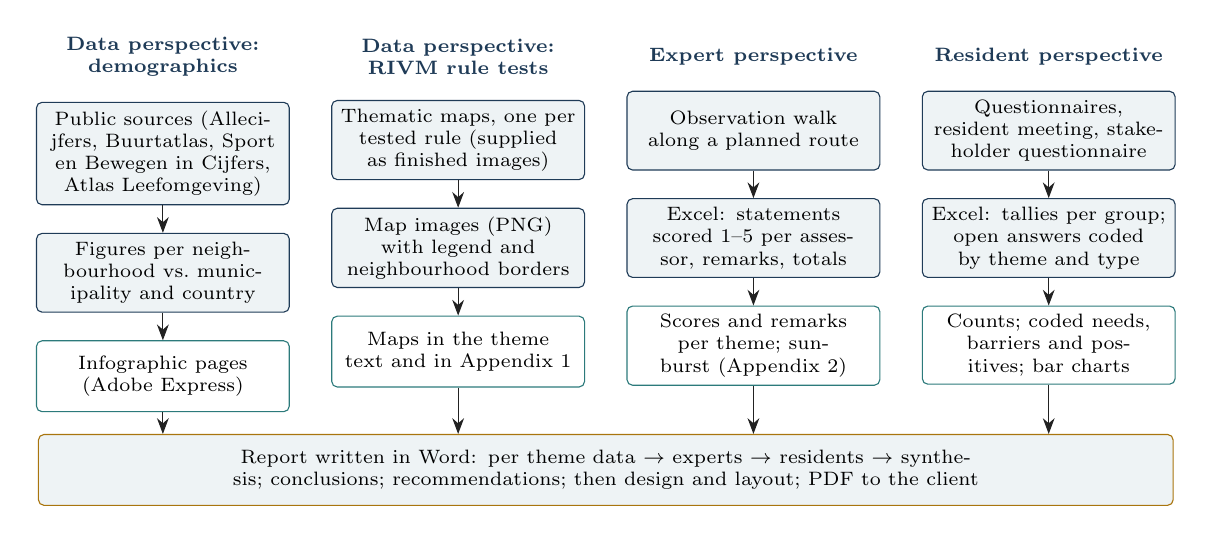
\begin{tikzpicture}[
  font=\scriptsize,
  box/.style={draw=navy, fill=light, rounded corners=2pt, align=center, text width=3.0cm, minimum height=1.0cm, inner sep=3pt},
  resbox/.style={draw=teal, fill=white, rounded corners=2pt, align=center, text width=3.0cm, minimum height=0.9cm, inner sep=3pt},
  rep/.style={draw=amber, fill=light, rounded corners=2pt, align=center, text width=14.2cm, minimum height=0.9cm, inner sep=3pt},
  lab/.style={font=\scriptsize\bfseries, text=navy, align=center, text width=3.2cm},
  arr/.style={-{Stealth[length=2mm]}, draw=inkgray}
]
\node[lab] (hD) at (0,0) {Data perspective:\\demographics};
\node[lab] (hM) at (3.75,0) {Data perspective:\\RIVM rule tests};
\node[lab] (hE) at (7.5,0) {Expert perspective};
\node[lab] (hR) at (11.25,0) {Resident perspective};
\node[box, below=0.2cm of hD] (d1) {Public sources (Allecijfers, Buurtatlas, Sport en Bewegen in Cijfers, Atlas Leefomgeving)};
\node[box, below=0.2cm of hM] (m1) {Thematic maps, one per tested rule (supplied as finished images)};
\node[box, below=0.2cm of hE] (e1) {Observation walk along a planned route};
\node[box, below=0.2cm of hR] (r1) {Questionnaires, resident meeting, stakeholder questionnaire};
\node[box, below=0.35cm of d1] (d2) {Figures per neighbourhood vs.\ municipality and country};
\node[box, below=0.35cm of m1] (m2) {Map images (PNG) with legend and neighbourhood borders};
\node[box, below=0.35cm of e1] (e2) {Excel: statements scored 1--5 per assessor, remarks, totals};
\node[box, below=0.35cm of r1] (r2) {Excel: tallies per group; open answers coded by theme and type};
\node[resbox, below=0.35cm of d2] (d3) {Infographic pages (Adobe Express)};
\node[resbox, below=0.35cm of m2] (m3) {Maps in the theme text and in Appendix 1};
\node[resbox, below=0.35cm of e2] (e3) {Scores and remarks per theme; sunburst (Appendix 2)};
\node[resbox, below=0.35cm of r2] (r3) {Counts; coded needs, barriers and positives; bar charts};
\node[rep, below=0.6cm of $(m3.south)!0.5!(e3.south)$] (w) {Report written in Word: per theme data $\rightarrow$ experts $\rightarrow$ residents $\rightarrow$ synthesis; conclusions; recommendations; then design and layout; PDF to the client};
\foreach \a/\b in {d1/d2,d2/d3,m1/m2,m2/m3,e1/e2,e2/e3,r1/r2,r2/r3} \draw[arr] (\a) -- (\b);
\foreach \a in {d3,m3,e3,r3} \draw[arr] (\a.south) -- (\a.south |- w.north);
\end{tikzpicture}
\caption{How a Wijkscan report is built today, as far as the reference report and its dataset show. Shaded boxes are collection and processing steps; white boxes are what reaches the report. Tools are named only where the files show them (Excel and Word files; Adobe Express in the infographics' metadata). Who does each step is not documented in this material.}\label{fig:process}
\end{figure}

Two documents of writing rules came with the synthetic dataset. One is an internal writing guide dated November 2025. Its checklist asks for a message that fits in one sentence, B1-level language, sentences of at most 20 words, active voice, the essence first, and one topic per paragraph. The other is a list of ten textual rules: factually accurate, clear, suited to the audience, concise, free of errors, logically structured, active, concrete, without needless repetition, and with a clear purpose.

The files of the reference case carry dates in their names or metadata:
\begin{itemize}
\item the expert results: March 2026;
\item the online sources: consulted on 1 April 2026;
\item the maps: 6 and 13 May 2026;
\item the sunburst: May 2026;
\item the inspiration map: 9 June 2026;
\item the final PDF: 23 June 2026.
\end{itemize}

\subsection{Where the time and the judgement go}\label{sec:process-effort}

My notes of the first stakeholder meeting record the following:
\begin{itemize}
\item expert data is collected in Excel files;
\item residents' responses are written down and connected with Excel;
\item analysing and interpreting all this data takes a lot of time;
\item project data is stored as local files in OneDrive, and a database was under construction;
\item around five people would use a tool like this.
\end{itemize}
My survey (Section~\ref{sec:res-survey}) puts numbers on this. Four of five respondents spend 21 hours or more per project on analysis and reporting. Qualitative analysis/coding and writing findings were each named twice as the most time-consuming part. Expert judgement is needed most for conclusions and recommendations, for combining the different kinds of data, for the qualitative data, and for finding and verifying sources. Researchers already draft with Microsoft Copilot, but its output cannot be traced back to the data (Section~\ref{sec:gap}).

\subsection{What this means for the system}\label{sec:process-implications}

Table~\ref{tab:report-sources} sets each element of the report against the files it comes from, and against whether a tool can trace it. Three consequences follow, and they shape the rest of this review.
\begin{enumerate}
\item \textbf{Most of the evidence is in spreadsheets.} Scores, remarks, coded answers and survey counts can be cited down to the cell. This is the case the citation-grounding literature in Section~\ref{sec:results} covers.
\item \textbf{The rule tests are in images.} The data perspective's central statements are made by reading maps, so a text-only pipeline cannot ground them. The tool has to analyse the supplied maps the way the reference report does. Section~\ref{sec:res-maps} reviews the literature on that, and Section~\ref{sec:m-maps} the method I adopt.
\item \textbf{Part of the report is not in any file.} Field photos, observations that never reached a spreadsheet, the outcomes of the resident meeting, the project context and literature all come from the research team. In a sample of 54 factual statements from the reference report's results chapter, 9 (17\%) relied on such knowledge. A traceable system must let the team record that knowledge with a source rather than invent it. The recommendations stay with the researcher, which matches the survey: only one of five respondents wants AI-drafted recommendations.
\end{enumerate}

\begingroup\renewcommand{\arraystretch}{1.3}
\begin{longtable}{|>{\raggedright\arraybackslash}p{3.6cm}|>{\raggedright\arraybackslash}p{5.4cm}|>{\raggedright\arraybackslash}p{5.2cm}|}
\caption{Elements of the reference report, their source in InnoBeweegLab's files, and whether a tool can trace them to that source.}\label{tab:report-sources}\\
\hline
\cellcolor{navy}\textcolor{white}{\textbf{Report element}} & \cellcolor{navy}\textcolor{white}{\textbf{Source in the files}} & \cellcolor{navy}\textcolor{white}{\textbf{Traceable by a tool?}} \\ \hline
\endfirsthead
\hline
\cellcolor{navy}\textcolor{white}{\textbf{Report element}} & \cellcolor{navy}\textcolor{white}{\textbf{Source in the files}} & \cellcolor{navy}\textcolor{white}{\textbf{Traceable by a tool?}} \\ \hline
\endhead
Theme sections: experts & scores and remarks in the expert workbooks & yes, to the cell \\ \hline
\rowcolor{light}
Theme sections: residents and stakeholders & tallies and coded answers in the resident workbook & yes, to the cell \\ \hline
Bar charts & survey tallies & yes; the chart can be redrawn from the counts \\ \hline
\rowcolor{light}
RIVM rule tests & map images & only if the tool measures the map (Sections~\ref{sec:res-maps}, \ref{sec:m-maps}) \\ \hline
Demographics & infographic images; the figures behind them are not in the dataset & only by reading the image, with confirmation by the researcher \\ \hline
\rowcolor{light}
Sunburst & totals workbook & yes; the chart is drawn from the workbook \\ \hline
Field photos, walk observations not in a sheet, resident meeting, project context, literature & not in the files & only if the team records them with a source \\ \hline
\rowcolor{light}
Recommendations & the researcher's judgement, inspiration pictures & not generated; written by the researcher \\ \hline
\end{longtable}
\endgroup

\clearpage
\section{Background}\label{sec:background}

\subsection{The field, and how it got here}\label{sec:field}

Citation-grounded generation descends from \textbf{Retrieval-Augmented Generation (RAG)} (Lewis et al., Facebook AI, NeurIPS 2020), which paired a parametric sequence-to-sequence model with non-parametric retrieval over a dense vector index specifically to make generation more factually grounded — the conceptual ancestor of nearly every method surveyed below. Three waves followed. First, \textbf{post-hoc correction} (RARR, 2022): let a model generate freely, then research and patch unsupported claims afterward. Second, \textbf{training the model itself to cite} (Self-RAG, 2024; FLARE, 2023): rather than always retrieving fixed passages, the model learns when to retrieve and emits citations and self-critique as part of generation. Third, \textbf{structured extraction before generation} (Auto-TA, GATOS, 2025): for qualitative-analysis use cases specifically, don't generate free text first — extract claims/codes tied to a source ID \textit{as the first step}, so traceability is built into the data structure rather than bolted onto the output. InnoBeweegLab's own pipeline (UC1's \texttt{SourceRecord} with a precise \texttt{locator} field, already implemented — see \texttt{innoweegbeg-ingestion}) follows this third pattern. In parallel, \textbf{automated factuality evaluation} matured from binary human judgments to fine-grained, atomic-fact decomposition (FActScore, RAGAS, SAFE, 2023–2024) precise enough to replace much of the cost of human evaluation, and \textbf{production-system audits} (CJR/Tow Center, Stanford RegLab, \textquotedblleft{}Cited but Not Verified\textquotedblright{}) started documenting, repeatedly, that shipped citation features are not as reliable as they look.



\subsection{Research gap and motivation}\label{sec:gap}

Four limitations in the literature motivate my thesis's specific angle:



\begin{enumerate}
\item \textbf{Citation presence $\neq$ citation correctness}, and this is not a minor edge case — it is the single most consistent finding across every production-system audit reviewed (Section~\ref{sec:res-production}): 37–94\% error rates across generative search engines (CJR/Tow Center), >17\% hallucination despite \textquotedblleft{}hallucination-free\textquotedblright{} marketing in legal AI (Stanford RegLab), and factual accuracy as low as 39\% in deep-research agents even when link-validity is 94\%+ (\textquotedblleft{}Cited but Not Verified\textquotedblright{}). A system that merely attaches a citation to every sentence has not solved traceability; it has to be independently verified, not assumed.
\item \textbf{LLM-as-judge verification is itself imperfect.} AttributionBench found even fine-tuned models plateau around 80\% macro-F1 at judging whether a citation supports a claim, and a bigger model (GPT-4) barely helped — meaning my evaluation design cannot rely purely on an LLM judge and needs either a structural/rule-based layer, human spot-checking, or both. Section~\ref{sec:res-evalmethod} surveys the broader literature on exactly why LLM-judges are unreliable and how that unreliability is measured, rather than treating this as a one-off finding from a single benchmark.
\item \textbf{Local, zero-budget, traceable pipelines are a thin, citable gap.} Of the 27+ systems reviewed, only GATOS (Katz et al.) and its Nature HSSC 2026 peer-reviewed version are open-weight/locally-runnable; both were validated only on synthetic case-study data. A separate EDM 2025 paper (Kim et al.) applied the same GATOS workflow to real qualitative data, narrowing but not closing this gap — it still used hosted DeepSeek inference rather than a zero-budget, fully local setup. No system reviewed combines open-weight, locally-runnable, \textit{and} real-data-validated. Every other citation-grounding and factuality-evaluation method in the literature (ALCE, Self-RAG, FActScore, RAGAS, SAFE, AttributionBench) is demonstrated against hosted, typically large, models with no RAM/hardware constraint discussed at all. This is precisely InnoBeweegLab's situation (16GB RAM, no dedicated GPU, zero budget) and precisely what my thesis is positioned to fill — a traceable report-generation pipeline \textit{validated on real, if anonymised, InnoBeweegLab data}, not just synthetic benchmarks.
\item \textbf{Images are outside the traceability methods reviewed.} Every citation-grounding and factuality method above grounds text in text. InnoBeweegLab's data perspective, however, reaches the report as map images and infographics (Section~\ref{sec:process}). Vision-language models read printed numbers well, but they are weakest at exactly the spatial judgements those maps encode, such as whether a building lies inside a distance zone (Section~\ref{sec:res-maps}). A traceable pipeline therefore needs a way to turn a supplied map into citable evidence, which none of the reviewed systems provides.
\end{enumerate}

\begin{calloutbox}{teal}{Field-phase finding}

Beyond the literature, I have direct field evidence the gap is real, not hypothetical: InnoBeweegLab's researchers already use the Microsoft Copilot desktop app to draft reports, but report that its output cannot be traced back to source data, and — per my own stakeholder survey (Section~\ref{sec:res-survey}) — traceability and human review score among the highest-importance items of anything I asked about, even though almost nobody flags tracing sources as a \textit{current} problem.

\end{calloutbox}

\subsection{Key overview figures}\label{sec:figures}

\textbf{Figure 1 — The field, by decomposition strategy and deployment context.} The methods below either decompose generation into independently-verifiable atomic units or they don't, and they are validated either against production/hosted-scale deployments or against something closer to InnoBeweegLab's local, zero-budget constraint. Nearly everything sits in the top-right; almost nothing sits in the bottom-right — which is exactly the gap Section~\ref{sec:gap} names.



\begingroup\renewcommand{\arraystretch}{1.3}
\begin{longtable}{|>{\raggedright\arraybackslash}p{3.4cm}|>{\raggedright\arraybackslash}p{5.5cm}|>{\raggedright\arraybackslash}p{5.5cm}|}
\hline
\cellcolor{navy}\textcolor{white}{\textbf{}} & \cellcolor{navy}\textcolor{white}{\textbf{Decomposes into atomic claims/codes}} & \cellcolor{navy}\textcolor{white}{\textbf{Does not decompose (whole-answer judgment)}} \\ \hline
\endfirsthead
\hline
\cellcolor{navy}\textcolor{white}{\textbf{}} & \cellcolor{navy}\textcolor{white}{\textbf{Decomposes into atomic claims/codes}} & \cellcolor{navy}\textcolor{white}{\textbf{Does not decompose (whole-answer judgment)}} \\ \hline
\endhead
\textbf{Validated at production/hosted scale} & ALCE $\cdot$ FActScore $\cdot$ RAGAS $\cdot$ SAFE $\cdot$ AttributionBench $\cdot$ PaperTrail $\cdot$ Auto-TA $\cdot$ Anthropic Citations API & RARR $\cdot$ Self-RAG $\cdot$ FLARE $\cdot$ CJR/Tow Center audit $\cdot$ Stanford RegLab study \\ \hline
\rowcolor{light}
\textbf{Validated local/zero-budget or small-scale} & GATOS $\cdot$ Nature HSSC 2026 $\cdot$ \textit{(my own evaluation harness, Section~\ref{sec:m-harness})} & \textit{(no method found)} \\ \hline
\end{longtable}
\endgroup

\textbf{Figure 2 — The convergent verification pattern.} Regardless of single-pass vs. multi-agent architecture (SQ3's open empirical question — see Section~\ref{sec:m-reference}), every rigorous method in Figure 1's left column follows the same four-step shape:



\begin{calloutbox}{amber}{Pipeline pattern}

\centering Ingest source data $\rightarrow$ Draft claims $\rightarrow$ Decompose into atomic, independently-checkable units $\rightarrow$ Verify each unit against its source $\rightarrow$ (Human validates before publishing)

\end{calloutbox}

This is the architecture InnoBeweegLab's own pipeline already follows by construction (UC1's \texttt{SourceRecord.locator}), and it is why the evaluation harness I built for this thesis (Section~\ref{sec:m-harness}) scores at the level of individual claims and their cited source-record ids, not whole-document judgments. The fully implemented version of this pipeline — with built (UC1) vs. planned (UC2–UC6) stages marked — is specified directly in the Requirements Engineering deliverable's domain/data model (SourceRecord $\rightarrow$ Claim $\rightarrow$ verification loop).



\subsection{Relevant concepts and definitions}\label{sec:definitions}

\begin{itemize}
\item \textbf{Traceability} — the property that every claim in a generated report can be followed back to the specific source row, cell, or image it came from (my research question's central term; operationalised in UC1 as the \texttt{SourceRecord.locator} field).
\item \textbf{Grounding / citation-grounding} — forcing generated text to be derivable from, and attributed to, specific supplied source material rather than the model's parametric memory (ZeroEntropy's practitioner taxonomy, grey-literature review \S1.2).
\item \textbf{Faithfulness} — the fraction of a text's atomic claims that are fully supported by its cited source(s) (RAGAS/FActScore's definition; implemented structurally in \texttt{src/evaluation/metrics.py}'s \texttt{faithfulness} function).
\item \textbf{Citation precision / recall} — of the ids a claim cites, what fraction are correct (precision); of the ids that actually support a claim, what fraction were cited (recall) (ALCE's definitions).
\item \textbf{Hallucination vs. misgrounding vs. fabrication} — a hallucination is any factually unsupported claim; Stanford RegLab's operational split distinguishes \textbf{misgrounding} (a real citation is given, but it doesn't actually support the claim) from what my evaluation harness calls \textbf{fabrication} (no citation is given at all). The two have different causes and different fixes, so they are scored separately rather than pooled into one \textquotedblleft{}hallucination rate.\textquotedblright{}
\item \textbf{Atomic claim decomposition} — breaking a generated text into its smallest independently-verifiable factual units before checking each one (FActScore's core method, also used by RAGAS, SAFE, PaperTrail, FacTool).
\item \textbf{RAG (Retrieval-Augmented Generation)} — generation conditioned on passages retrieved from an external corpus at inference time (Lewis et al., 2020).
\item \textbf{Single-pass vs. multi-agent pipeline} — whether report drafting is done by one model call (optionally with a built-in verification step) or by multiple specialised model calls/roles (e.g. a drafting agent and a separate grounding-checker agent, as in Auto-TA). SQ3 treats this as an open empirical question, not a premise (Section~\ref{sec:m-reference}).
\item \textbf{Human-in-the-loop validation} — a required manual approval/correction step before any AI-drafted claim is published (UC4 in the requirements doc; the design constraint that both PaperTrail and \textquotedblleft{}Hide or Highlight\textquotedblright{} found is harder to make effective than it sounds — see Section~\ref{sec:res-hitl}).
\item \textbf{LLM-as-judge} — using a language model itself to score another model's output (e.g. for faithfulness or relevance) rather than a human or a rule-based check; AttributionBench's $\sim$80\% F1 ceiling (Section~\ref{sec:gap}) is the key limitation to keep in mind whenever my own evaluation leans on it, and Section~\ref{sec:res-evalmethod} surveys the specific, named biases (position, verbosity, self-enhancement) documented for this technique.
\item \textbf{Vision-language model (VLM)} — a model that takes an image together with text as input and produces text, for example Qwen2.5-VL; used here to read printed numbers from infographics (Section~\ref{sec:res-maps}).
\item \textbf{Choropleth or thematic map} — a map on which areas or objects are coloured by class according to a legend; InnoBeweegLab's rule maps colour every building this way (Table~\ref{tab:rules-maps}).
\item \textbf{Extract-then-reason} — first converting an image into a structured table with a dedicated extractor, then reasoning over the table rather than over the pixels (MapQA's V-MODE, DePlot; Section~\ref{sec:res-maps}).
\item \textbf{Image registration} — aligning two images of the same scene so that their pixels correspond (Zitov\'a \& Flusser, 2003); used here to align a distance-zone map with a map that shows the same buildings (Section~\ref{sec:m-maps}).
\item \textbf{Evaluation protocol / evaluation methodology} — the overall design of \textit{what} is measured, \textit{where} (on which data/benchmark), and \textit{how} (automatic metric, human rating, or LLM-judge), plus the reporting practices (documented criteria, repeated runs, stated sample size) that make the result trustworthy and reproducible rather than a one-off number (Chang et al. 2024's framework; see Section~\ref{sec:res-evalmethod}).
\end{itemize}

\clearpage
\section{Relevant results}\label{sec:results}

\textit{What follows are the concrete findings from the literature that my own system and evaluation will be measured against, or will try to build on / improve on, organised by what each cluster of results is relevant to.}



\subsection{Citation-grounded / attributed generation methods — results relevant to \textit{which generation architecture to adopt}}\label{sec:res-generation}

\begin{itemize}
\item \textbf{RARR} (Google, 2022) — post-hoc: researches evidence via web search for any LLM's claims, edits unsupported text. Model-agnostic, few-shot. arXiv:2210.08726
\item \textbf{ALCE} (Princeton/Gao et al., EMNLP 2023) — benchmark + pipeline for citation generation. ChatGPT: 73.6\%/72.5\% citation recall/precision on ASQA, improving to 84.8\%/81.6\% with reranking; collapsed to $\sim$20\% on harder list-style QAMPARI task. \textquotedblleft{}Even the best models lack complete citation support 50\% of the time\textquotedblright{} on ELI5. \textbf{Relevance:} this is the precision/recall definition my evaluation harness implements structurally; the ASQA-vs-QAMPARI gap is a warning that citation quality is highly task-dependent, so InnoBeweegLab's own task shape must be tested directly rather than assumed from a generic benchmark. arXiv:2305.14627
\item \textbf{Self-RAG} (Asai et al., UW/AI2, ICLR 2024) — trains model to decide when to retrieve + emit self-critique \textquotedblleft{}reflection tokens\textquotedblright{} rather than always retrieving fixed passages. 13B model: 70.3\%/71.3\% citation precision/recall on ASQA vs. naive retrieval-augmented Llama2-13B at only 19.8\%/36.1\%. \textbf{Relevance: architecture/training for citation matters far more than bolting retrieval onto a normal LLM} — directly informs SQ3's architecture comparison. arXiv:2310.11511
\item \textbf{FLARE} (CMU, EMNLP 2023) — iterative, triggers retrieval only when the model is about to generate a low-confidence token. arXiv:2305.06983
\item \textbf{AIS framework} (Rashkin et al., Google, 2021) — formalized \textquotedblleft{}Attributable to Identified Sources\textquotedblright{} (AIS), a framework for judging whether generated text is attributable to given source material; published in \textit{Computational Linguistics} (MIT Press, 2023). The related \textbf{Attributed QA} benchmark (Bohnet et al., Google, 2022) applies this framework to open-domain QA with retrieval-augmented systems. arXiv:2112.12870 (AIS) / arXiv:2212.08037 (Attributed QA)
\item \textbf{FacTool} (Chern et al., 2023) — general claim-extraction $\rightarrow$ verification pipeline across QA/code/math/science. arXiv:2307.13528
\item \textbf{Chain-of-Verification (CoVe)} (Meta, ACL Findings 2024) — draft $\rightarrow$ generate independent verification questions $\rightarrow$ answer blind $\rightarrow$ revise. arXiv:2309.11495
\end{itemize}

\subsection{Automated factuality/faithfulness evaluation — results relevant to \textit{how well my own evaluation method can be trusted}}\label{sec:res-factuality}

\begin{itemize}
\item \textbf{FActScore} (UW/Meta, EMNLP 2023) — decomposes text into atomic facts, checks each against a KB. ChatGPT scored only \textbf{58\%} on biography generation. Automated estimator had <2\% error vs. human eval, at a fraction of the cost (\$26K human-eval cost avoided). arXiv:2305.14251 — \textit{re-verified directly against the arXiv abstract on 2026-10-07; this is also the paper the evaluation harness's \texttt{faithfulness} function (\texttt{src/evaluation/metrics.py}) is modelled on.}
\item \textbf{SummaC} (Laban et al., TACL 2022) — repurposes NLI models, sentence-pair aggregation. 74.4\% balanced accuracy, +5pts over prior methods. arXiv:2111.09525
\item \textbf{TRUE benchmark} (Google, NAACL 2022) — meta-evaluates factual-consistency metrics; NLI-based and QA-based approaches are strongest and complementary. arXiv:2204.04991
\item \textbf{RAGAS} (Es et al., EACL 2024) — open-source, industry-standard RAG evaluation. \textbf{Faithfulness} = claims supported by retrieved context / total claims. Also Context Precision/Recall auditing the retrieval step itself. Already used as evaluation framework in the Chalmers/Volvo thesis reviewed earlier (Section~\ref{sec:res-prior}). arXiv:2309.15217
\item \textbf{SAFE + LongFact} (Google DeepMind/Stanford, 2024) — atomic-decomposition grounded against live search. Agreed with human raters 72\% of the time; on disagreements, SAFE was correct 76\% of the time; >20x cheaper than human annotation. \textbf{Relevance:} strong evidence automated fact-checking can match/exceed human-rater reliability on a budget — directly supports using an automated harness as the primary evaluation method, with human spot-checks rather than full human re-grading. arXiv:2403.18802
\item \textbf{AttributionBench} (2024) — benchmarks whether LLMs can reliably judge if a citation supports a claim. Ceiling $\sim$80\% macro-F1 even for fine-tuned GPT-3.5; bigger model (GPT-4) didn't help much. See Section~\ref{sec:gap}. arXiv:2402.15089
\end{itemize}

\subsection{Production systems and audits — results relevant to \textit{what traceability failure actually looks like in deployed systems}}\label{sec:res-production}

\begin{itemize}
\item \textbf{Anthropic Citations API} (2025) — chunks source docs, attaches every response to source chunks. Case study (Endex): source hallucinations 10\%$\rightarrow$0\%, +20\% references/response. Vendor-reported.
\item \textbf{CJR/Tow Center audit} (2024/25) — 8 generative search engines, 1,600 queries. Perplexity 37\% incorrect; ChatGPT Search >60\% incorrect; Grok-3 94\% error rate. \textbf{Paid tiers were more confidently wrong than free tiers.}
\item \textbf{AlgorithmWatch Bing Chat study} (2023) — $\sim$30\% factual errors in election Q\&A; fabricated claims attributed to real, credible outlets — \textquotedblleft{}illusion of validity\textquotedblright{} via false attribution.
\item \textbf{Stanford RegLab legal-AI study} (2025, preregistered) — Lexis+ AI and Ask Practical Law AI both hallucinate in >17\% of responses despite \textquotedblleft{}hallucination-free\textquotedblright{} marketing. Source of the misgrounding/fabrication distinction used throughout this review (Section~\ref{sec:definitions}).
\item \textbf{Vals Legal AI Report} (2025) — Harvey/CoCounsel vs. practicing lawyers; Harvey 94.8\% on document Q\&A. Citation/traceability performance is highly task-dependent, not one global capability.
\item \textbf{Glean} — enterprise RAG, permission-aware, cites the Stanford legal numbers as rationale for grounding.
\item \textbf{\textquotedblleft{}Cited but Not Verified\textquotedblright{}} (2026) — 14 deep-research agents, 130 queries: link-validity 94\%+, topical-relevance 80\%+, factual-accuracy only \textbf{39–77\%}. Fact-checking accuracy degrades $\sim$42\% as agents take more search steps. \textbf{More citations per response correlated with LOWER factual accuracy.} Single most directly on-topic recent study for this thesis. arXiv:2605.06635
\end{itemize}

\subsection{Structured-extraction \& multi-agent report pipelines — results relevant to \textit{whether InnoBeweegLab's use case needs a multi-agent architecture}}\label{sec:res-pipelines}

\begin{itemize}
\item \textbf{Auto-TA} (2025) — closest analog to InnoBeweegLab's use case. Multi-agent qualitative-coding pipeline with a Quote ID on every code/theme. Credibility rose from 82.13\% baseline to \textbf{98.41\%} with a specialized persona + grounding-checker agent. arXiv:2506.23998
\item \textbf{SFT-TA} (2025) — fine-tuned agents underperform GPT-4o alone individually, but outperform both fine-tuned-single-agent and GPT-4o baseline once embedded in a multi-agent system. arXiv:2509.17167
\item \textbf{PublicAgent} (Montazeri, Feng \& Sha, 2026) — a multi-agent architecture for open-data analysis (intent clarification, data discovery, data analysis, report generation agents) tested via ablation across 8 LLMs and 50 benchmark queries: removing any single agent cost the full system 72–100\% of pairwise wins against the ablated version, and different agents failed in distinct, non-redundant ways — discovery/analysis-agent removal caused catastrophic failure (empty or nonsensical output), while report/intent-agent removal caused milder quality degradation. Specialisation improved results independent of the base model's own strength. \textbf{Relevance:} a finer-grained empirical picture for SQ3 than a single pass/fail verdict — discovery/analysis-type agents (handling data, closest to InnoBeweegLab's SourceRecord/ingestion layer) were consistently valuable, while report/intent-type agents were more model-dependent, echoing the caution the Chalmers/Volvo result (Section~\ref{sec:res-prior}) raises specifically for report-synthesis agents. doi.org/10.1016/j.dte.2026.100136
\item \textbf{GATOS Workflow} (Katz, Coloyan Fleming \& Main, 2024) — open-source, locally-runnable thematic-analysis pipeline (Llama-3.1-70B/8B, WizardLM2-8x22B, Mistral-22B/12B-nemo), explicitly avoiding cloud APIs for sensitive data. Validated only on three synthetic case-study datasets: fewer than 5\% of sub-themes had no clear match, under 2\% had no close match at all. arXiv:2410.03721
\item \textbf{Nature HSSC 2026} (Katz, Coloyan Fleming \& Main) — the peer-reviewed version of the GATOS workflow above, published in \textit{Humanities and Social Sciences Communications} 13, article 209.
\item \textbf{GATOS applied to real data} (Kim, Ke, Zhang \& Barrett, EDM 2025) — a separate paper applying the Katz et al. GATOS workflow to real (not synthetic) qualitative data, using DeepSeek + mxbai-embed-large-v1 embeddings, on a neurodiversity-support study (interviews with healthcare providers, teachers, caregivers). This narrows, but doesn't close, the real-data validation gap named below: it still used hosted inference, not InnoBeweegLab's 16GB-RAM, zero-budget, fully local constraint.
\item \textbf{PaperTrail} (CHI 2026) — bi-directional claim decomposition (both the LLM answer AND source docs), flags \textquotedblleft{}supported / unsupported / omitted.\textquotedblright{} arXiv:2602.21045
\end{itemize}

\subsection{Human-in-the-loop verification interface patterns — results relevant to \textit{designing the Workshop-phase review interface}}\label{sec:res-hitl}

\begin{itemize}
\item \textbf{PaperTrail} (CHI 2026) — 26 scholars, within-subjects study. Structured claim-evidence UI \textbf{lowered trust appropriately but did NOT change verification behavior} — reviewers still mostly accepted LLM edits.
\item \textbf{\textquotedblleft{}Hide or Highlight\textquotedblright{}} (AIES 2025/26, N=148) — hiding/vaguing uncertain content produced \textit{higher and more appropriate} trust than highlighting it (appropriate compliance: 90\% Ambiguity / 86\% Opaque vs. only 66\% Transparent highlighting).
\item \textbf{AutoUAT / Test Flow} (Ferreira, Viegas, Faria \& Lima, 2025 industrial case study) — a two-step LLM pipeline generating acceptance-test scenarios (95\% rated helpful by product owners, across 166 real usage instances) and executable test scripts (60\% usable as generated, rising to 92\% with minor fixes) from user stories, deployed in an automotive-industry workflow with mandatory human review before any generated test merges. Different domain from report generation, but the same pattern as PaperTrail/\textquotedblleft{}Hide or Highlight\textquotedblright{}: generated output is treated as a draft a human must approve, not a final artefact — directly supporting UC4's human-in-the-loop requirement. The tool's output also once surfaced a real application defect the generated test scenario had flagged but the human team hadn't noticed, a concrete example of traceable AI output adding value beyond pure time-saving. arXiv:2504.07244
\item Broader CSCW/CHI literature: showing confidence scores doesn't reliably improve human error-catching, and can increase over-reliance.
\end{itemize}

\subsection{Prior comparable work — results relevant to \textit{hardware and architecture feasibility specifically}}\label{sec:res-prior}

\begin{itemize}
\item The \textbf{Chalmers/Volvo master's thesis} (Nihlstrand \& Lundberg, 2025, multi-agent LLM system for automated report generation from unstructured logbooks) used Phi-4 (14B), LLaMA-3.3-70B and GPT-4o, all via hosted inference, and found its multi-agent system scored \textit{worse overall} than a naive single-pass baseline (3.60/7 vs 3.78/7), only beating it on factuality specifically. It also found RAG/retrieval grounding — not raw model size — was the biggest lever on factuality in its own ablation study, which this review's own findings (Section~\ref{sec:res-generation}, Self-RAG) independently corroborate. It did not validate laptop-class local deployment at all; a 70B model is far outside InnoBeweegLab's 16GB-RAM laptop.
\end{itemize}

\subsection{Systematic evaluation methodology as its own field of study — results relevant to \textit{designing a trustworthy evaluation protocol in general, not just assembling a project-specific checklist}}\label{sec:res-evalmethod}

Sections~\ref{sec:res-generation}--\ref{sec:res-prior} above answer \textquotedblleft{}which metrics and generation methods exist.\textquotedblright{} This subsection asks a different, prior question, raised directly by feedback that the methodology in Section~\ref{sec:m-reference} needed to read as literature-grounded research rather than an invented one-off: how does the literature say an evaluation \textit{protocol itself} should be designed? Four sub-threads of this field are directly relevant.



\textbf{Evaluation as a three-part design problem, not a single metric choice.} Chang et al.'s \textquotedblleft{}A Survey on Evaluation of Large Language Models\textquotedblright{} (arXiv:2307.03109, ACM TIST 2024) frames systematic evaluation of any generative system around three separable questions — \textit{what} to evaluate (which capabilities/tasks matter for the use case), \textit{where} to evaluate (which dataset/benchmark/gold set actually represents that use case), and \textit{how} to evaluate (automatic metric, human judgment, or LLM-as-judge, each with different cost/reliability trade-offs). \textbf{Relevance:} this is the structure Section~\ref{sec:m-reference} is implicitly following (what = traceability/faithfulness/content coverage; where = the frozen gold set plus the real Euterpepark report and a naive baseline; how = structural metrics + human rubric), but had not previously been named as a methodology choice in its own right.



\textbf{LLM-as-judge is its own well-studied sub-field, with documented, specific failure modes — not a generic \textquotedblleft{}AI checks AI\textquotedblright{} shortcut.} Gu et al.'s \textquotedblleft{}A Survey on LLM-as-a-Judge\textquotedblright{} (arXiv:2411.15594) proposes a formal reliability framework built on three axes — agreement with human judgment, susceptibility to bias, and adversarial robustness — and separates \textit{task-agnostic} biases (diversity, cultural, self-enhancement bias) from \textit{judgment-specific} ones (position, length/verbosity, style, concreteness bias). Zheng et al.'s earlier \textquotedblleft{}Judging LLM-as-a-Judge with MT-Bench and Chatbot Arena\textquotedblright{} (arXiv:2306.05685) is the empirical paper this taxonomy builds on, and measured these directly in GPT-4-as-judge setups: \textbf{position bias} (the judge favours whichever answer it sees first), \textbf{verbosity bias} (longer answers score higher independent of quality), and \textbf{self-enhancement bias} (a model judges its own outputs more favourably). Han et al.'s \textquotedblleft{}Judge's Verdict: A Comprehensive Analysis of LLM Judge Capability Through Human Agreement\textquotedblright{} (arXiv:2510.09738, 2025) goes further, arguing a judge should not be trusted on its raw score at all — it should first be benchmarked against a measured human-agreement rate, the way a new diagnostic test is validated against a gold standard before deployment. \textbf{Relevance:} this is the literature-level grounding for a decision already made implicitly in Section~\ref{sec:gap} (point 2) and Section~\ref{sec:m-harness} — that an LLM-judge component in my evaluation harness cannot be trusted at face value — and it means any future LLM-judge step added to \texttt{src/evaluation/} needs either a structural cross-check or its own measured agreement rate against InnoBeweegLab's human reviewer, not just a plausible-sounding prompt.



\textbf{Reproducibility is a methodology in itself, with known, specific pitfalls.} Biderman et al., \textquotedblleft{}Lessons from the Trenches on Reproducible Evaluation of Language Models\textquotedblright{} (arXiv:2405.14782, EleutherAI, authors of the widely-used \texttt{lm-eval} harness) document — from three years of running a shared evaluation framework across the field — that evaluation results are routinely non-reproducible because of unreported \textquotedblleft{}minor\textquotedblright{} implementation details (prompt formatting, answer-extraction rules), shifting conventions, and social incentives to under-report negative or inconvenient results. Their recommended fixes: release the evaluation code itself, document the exact methodology, report variance across multiple repeated runs rather than a single score, and run exploratory error analysis rather than just a headline number. \textbf{Relevance:} this is the literature precedent for practices my harness already follows by construction (\texttt{src/evaluation/} is itself the released evaluation code; \texttt{runner.py}/\texttt{results\_log.py} already log mean$\pm$stdev across repeats, per Section~\ref{sec:m-harness}) — the earlier draft of this review had adopted the practice without citing why it is good practice.



\textbf{Human evaluation has its own, separately-documented best-practice literature — and the field frequently fails to follow it.} Van der Lee et al.'s \textquotedblleft{}Best practices for the human evaluation of automatically generated text\textquotedblright{} (INLG 2019) is the foundational checklist for designing a human-rater study of generated text: pre-registering evaluation criteria, piloting the rating instrument, reporting rater demographics/training, and reporting inter-rater agreement. Mei et al.'s \textquotedblleft{}Illusions of the Gold Standard: A Large-scale Analysis of Human Evaluation Protocols for Long-form Text Generation\textquotedblright{} (arXiv:2606.07936, 2026) is a direct, large-scale check on whether the field actually follows that checklist: across 284 manually-annotated *CL papers (2023–2025) plus 1,800+ more, \textquotedblleft{}only around half... include guidelines for human evaluation tasks,\textquotedblright{} and \textbf{no paper in the sample reported a power analysis to justify its sample size.} \textbf{Relevance:} this is a direct warning for Section~\ref{sec:m-reference}'s human-rubric step — as originally drafted, that step did not state its own evaluation guidelines, rater qualification, or sample-size justification in writing, which is exactly the gap Mei et al. find in roughly half of the published literature. Section~\ref{sec:m-reference} is revised below to close this specific gap rather than repeat it.



\subsection{Field-phase evidence: my own InnoBeweegLab stakeholder survey (n=5) — results relevant to validating the research gap and sharpening the main research question}\label{sec:res-survey}

Everything in Sections~\ref{sec:res-generation}--\ref{sec:res-evalmethod} is literature or production-system evidence from outside InnoBeweegLab. This subsection is different: it is primary field data I collected myself, a \textquotedblleft{}Research \& Reporting Workflow Survey\textquotedblright{} distributed to InnoBeweegLab researchers, coordinators, and project leads via Microsoft Forms. As of 7 October 2026 it has 5 responses and remains open, so the numbers below are indicative at this sample size, not final — I will re-run this analysis with the full response set before the final report. Two individual questions (data types normally worked with; difficulty combining qual/quant/expert findings) returned data that looks like a Forms display quirk rather than a real signal (nearly every respondent selected \textquotedblleft{}Other\textquotedblright{} on a straightforward multiple-choice data-type question) and are flagged rather than reported as findings.



\textbf{Workload and pain points.} The analysis-and-reporting phase is a real time cost: 4 of 5 respondents spend 21+ hours per project on it (2 at 21–40h, 2 at more than 40h), and for 3 of 5 the writing/structuring step alone takes 11–20 hours. Combining information from different data sources takes 2–10 hours for most respondents. Ranked by how many respondents flagged each as a current problem (of 5, multi-select): \textquotedblleft{}Writing reports takes too much time\textquotedblright{} and \textquotedblleft{}Maintaining consistency across reports\textquotedblright{} tie at 4; \textquotedblleft{}Data is stored in different formats\textquotedblright{} and \textquotedblleft{}Reports require significant rewriting\textquotedblright{} tie at 3; \textquotedblleft{}Combining sources is difficult\textquotedblright{} and \textquotedblleft{}Analysis takes too much time\textquotedblright{} tie at 2; \textquotedblleft{}It is difficult to trace conclusions back to evidence\textquotedblright{} scored only 1 — the lowest item on the list.



\begin{calloutbox}{amber}{Design implication}

Traceability and human control: not today's complaint, but tomorrow's requirement. That last number is worth pausing on, because what respondents say they currently struggle with and what they say actually matters point in opposite directions. Asked directly how important it is that every AI-generated conclusion can be traced back to its supporting evidence, the average score was \textbf{4.8 out of 5}; asked how important it is that a researcher can review, edit, approve, or reject AI-generated content before it becomes part of a report, the average was a perfect \textbf{5.0 out of 5} — unanimous. Read together with the problem-ranking above, the finding is: nobody is struggling to trace sources today because nobody is really attempting AI-assisted drafting yet. Traceability and human control are not reported pain points, they are the non-negotiable condition for adopting a new tool at all — exactly the premise my main research question is built on, now with quantified stakeholder backing rather than a single anecdote (Section~\ref{sec:gap}).

\end{calloutbox}

\textbf{What respondents want — and don't want — from an AI-supported tool.} Four functions got unanimous (5/5) support: analysing Excel/quantitative data, summarising interviews or qualitative responses, identifying themes and patterns, and comparing findings across multiple data sources — exactly the synthesis-heavy steps the workload data above says cost the most hours. Interest drops for \textquotedblleft{}generate draft findings/conclusions\textquotedblright{} (3/5 each), drops further for \textquotedblleft{}generate draft recommendations\textquotedblright{} (1/5): respondents want help synthesising evidence, not help deciding what to recommend. \textquotedblleft{}Supporting review and editing of generated content\textquotedblright{} scored 0/5, which — read against the 5.0/5 importance score above — looks like respondents treat human review as an assumed baseline rather than a feature worth asking for, not as something nobody wants.



\textbf{What they're worried about — and what they're not.} Top concerns, by how many respondents flagged each: incorrect information, unsupported conclusions/hallucinations, and generic recommendations each scored 4/5, followed by important context being missed and bias at 3/5 each. Compliance-style concerns scored far lower: privacy/GDPR, data security, and lack of transparency each got only 1/5. Respondents are worried about the system being \textit{wrong}, not about it being \textit{unsafe to use} — a direct steer toward where the evaluation-methodology work in Sections~\ref{sec:res-evalmethod} and~\ref{sec:m-reference} should concentrate its rigour.



\textbf{A concrete success bar, in their own words.} Asked what reduction in analysis/reporting time would make such a system worthwhile, 3 of 5 said 25–50\% and 2 of 5 said 10–25\%; nobody asked for more than 50\%. That is a real, stakeholder-stated number I can fold into the \textquotedblleft{}most efficient, cost-effective, and highest-value\textquotedblright{} framing of my main research question. Free-text answers reinforce the same theme on both sides: what would build trust is seeing \textquotedblleft{}on which data the recommendation is based\textquotedblright{} and knowing \textquotedblleft{}the sources actually check out\textquotedblright{}; what would make the system unacceptable is \textquotedblleft{}mistakes in the conclusions,\textquotedblright{} or — as one respondent put it — if \textquotedblleft{}correcting/checking the AI data costs more time than writing it ourselves,\textquotedblright{} which sets a hard floor under the time-savings number above.



4 of 5 respondents are willing to participate in a follow-up interview, and all 5 are willing to test and evaluate a prototype later in the project — concrete recruitment for the Phase 4 stakeholder evaluation (Section~\ref{sec:m-reference}) this report's own evaluation methodology depends on.



\subsection{Maps, charts and infographics as evidence --- results relevant to \textit{analysing the map inputs the way the reference report does}}\label{sec:res-maps}

Every method in Sections~\ref{sec:res-generation}--\ref{sec:res-pipelines} grounds text in text. None of them cites a region of an image. Yet InnoBeweegLab's data perspective reaches the report as images (Section~\ref{sec:process-perspectives}):
\begin{itemize}
\item maps on which the answer to an RIVM rule is a colour per building, a distance zone, or a marker;
\item infographics with printed numbers;
\item a sunburst chart.
\end{itemize}
The user supplies the maps as finished images, so the tool has to read them. This subsection collects what the literature says about reading such images automatically, and how reliable that is.

\begin{itemize}
\item \textbf{Local vision-language models read printed text and numbers well.} The Qwen2.5-VL technical report (Bai et al., 2025) gives its 7B model 95.7 on DocVQA, 87.3 on ChartQA and 82.6 on InfoVQA. A 7B model is in the same size class as the drafting models considered for the 16GB-RAM laptop. ChartQA (Masry et al., 2022) is a benchmark of 9.6K human-written and 23.1K generated questions about charts. The same model reports bounding boxes and points in the coordinates of the input image, which would let a reading point to the image region it came from. \textbf{Relevance:} the numbers printed on InnoBeweegLab's demographic infographics are within reach of a laptop-class model.
\item \textbf{The same models fail at simple spatial judgements.} \textquotedblleft{}Vision language models are blind\textquotedblright{} (Rahmanzadehgervi, Bolton, Taesiri \& Nguyen, ACCV 2024) tested four frontier models (GPT-4o, Gemini-1.5 Pro, Claude-3 Sonnet, Claude-3.5 Sonnet) on visual tasks that are easy for people. Their average accuracy was:
\begin{itemize}
\item 56.84\% on whether two lines intersect;
\item 39.44\% on counting overlapping circles;
\item 48.90\% on following single-coloured paths;
\item 58.07\% across all tasks, against 24\% for random guessing.
\end{itemize}
The authors trace the failures to how images are tokenised, and name checking whether streets intersect on a map as a real-world consequence. \textbf{Relevance:} \textquotedblleft{}does this building lie inside the 200\,m zone?\textquotedblright{} is exactly this kind of judgement.
\item \textbf{Map reasoning is an open problem.} MapBench (Xing et al., 2025) poses 1,649 path-finding queries on 100 maps of nine types. Under both zero-shot and chain-of-thought prompting, it \textquotedblleft{}significantly challenges\textquotedblright{} Llama-3.2-11B-Vision, Qwen2-VL-7B, GPT-4o and GPT-4o mini. MapEval (Dihan et al., ICML 2025) asks 700 questions about maps of 180 cities in 54 countries and tests 30 foundation models. No model exceeds 67\% accuracy, all trail humans by more than 20 percentage points, and they are weakest on distances, directions and routes.
\item \textbf{Extracting first and reasoning second works far better than asking the model directly.} MapQA (Chang, Palzer, Li, Fosler-Lussier \& Xiao, NeurIPS 2022 TRL workshop) builds a dataset of 62,367 choropleth maps with 795,525 questions. Its V-MODE method first extracts the map's underlying data, the value of every region, into a table, and only then answers questions over that table. For maps with a discrete legend the extraction reaches 92.0--99.9\% accuracy. Question answering on top of the table beats end-to-end baselines: on the MapQA-S subset (with oracle text recognition) it scores 87.1, against 72.2 for the best baseline and 89.8 for humans. DePlot (Liu et al., Findings of ACL 2023) applies the same idea to charts: it first translates a plot into a table, then lets a language model reason over it. This improves on the fine-tuned state of the art by 29.4\% on human-written ChartQA questions.
\item \textbf{Repeated readings can be turned into an uncertainty signal.} Self-ensembling (Berkane, Wang \& Majumder, 2026) prompts the same vision-language model several times on one chart, aligns the resulting tables, and takes the median of every cell. On a chart-extraction benchmark this improves accuracy by up to 8.09 points (about 23\% relative). The spread between readings correlates with error (Spearman $\rho$ between $-0.30$ and $-0.37$), which the authors present as a heuristic uncertainty measure, not a calibrated probability.
\item \textbf{Working on the GIS data instead of the picture.} Autonomous GIS (Li \& Ning, 2023) uses GPT-4 as a reasoning engine that runs GIS operations on spatial data (data collection, analysis, mapping) and produced correct results in three case studies. This is the stronger route when vector data is available. It does not fit this project, because it depends on a hosted model and InnoBeweegLab's input to the reporting step is the finished map image.
\end{itemize}

\begin{calloutbox}{teal}{Relevance for InnoBeweegLab}

The decisive information on InnoBeweegLab's maps is encoded in colour per building, in distance zones and in markers (Table~\ref{tab:rules-maps}). Those are the fine spatial judgements vision-language models get wrong. The infographics, by contrast, carry printed numbers, which these models read well. The literature therefore points to a split. The maps should be measured deterministically by reading the legend into a table, as in MapQA and DePlot. Model reading should be kept for printed numbers, with repeated readings and a human check (Section~\ref{sec:res-hitl}). Section~\ref{sec:m-maps} describes how I apply this.

\end{calloutbox}

\clearpage
\section{Inspiring methodologies}\label{sec:methods}

\textit{Methods and best practices I found in the literature (and, where explicitly noted, in the grey-literature review) that I am adopting directly in my own design — and why.}



\subsection{Atomic-claim decomposition + automated scoring, logged over repeated runs}\label{sec:m-harness}

RAGAS, FActScore, and SAFE all score generation by decomposing it into atomic claims and checking each independently; Inspect AI and DeepEval generalise this into a reusable harness pattern (frozen test set + automated scoring + logged runs); \textquotedblleft{}Do Repetitions Matter?\textquotedblright{} (arXiv:2509.24086) adds that LLM stochasticity means a single run per condition risks mistaking noise for a real difference — the same point Biderman et al. make at the level of an entire evaluation field (Section~\ref{sec:res-evalmethod}). \textbf{This is interesting to me because it is exactly the harness already implemented} (\texttt{src/evaluation/} — \texttt{metrics.py} for the atomic-claim scoring, \texttt{runner.py} for repeated runs per condition, \texttt{results\_log.py} for mean$\pm$stdev logging across runs) rather than an idea still to build. The one limitation carried over explicitly: these metrics are currently \textit{structural} proxies (they score \texttt{cited\_ids} already attached to a claim), because UC2 (draft generation) doesn't exist yet to produce real free text to decompose — the upstream LLM-judge extraction step is the documented next step once it does, and per Section~\ref{sec:res-evalmethod} it will need its own measured human-agreement check before being trusted, not just a plausible prompt.



\subsection{Provenance-by-construction, not provenance-by-retrofit}\label{sec:m-provenance}

Auto-TA's Quote ID (every code/theme carries a direct pointer to its transcript segment) and PaperTrail's bi-directional decomposition both build traceability into the data structure from the first processing step, rather than trying to attribute a already-generated block of text after the fact. \textbf{This is interesting to me because it is the same design principle UC1's \texttt{SourceRecord.locator} already follows} — every ingested row, cell, or image gets a precise locator at ingestion time, before any drafting happens — and it's the reason the evaluation harness's citation metrics are meaningful at all: there is nothing to misattribute if every unit already carries its true source id.



\subsection{Reference-and-baseline comparison — evaluating report quality against InnoBeweegLab's own human-written report, as an application of the general evaluation-methodology literature in \texorpdfstring{Section~\ref{sec:res-evalmethod}}{Section 4.7}}\label{sec:m-reference}

This answers \textquotedblleft{}how do I evaluate model performance for report generation, given data, to be as good as the real InnoBeweegLab report\textquotedblright{} — but, following feedback that this needed to be grounded research rather than an invented protocol, it is presented here explicitly as an \textit{application} of the general literature on systematic evaluation design (Section~\ref{sec:res-evalmethod}), not a one-off checklist for this project alone. Concretely: the \textit{what/where/how} structure (Chang et al., Section~\ref{sec:res-evalmethod}) is used to separate the three questions below; any LLM-judge component is treated as a measured, bias-prone instrument rather than a ground truth (Gu et al.; Zheng et al.; Judge's Verdict — Section~\ref{sec:res-evalmethod}); and the reproducibility and human-evaluation documentation practices below are stated explicitly, rather than left implicit, specifically to avoid the gap Mei et al. (Section~\ref{sec:res-evalmethod}) find in roughly half of published NLP evaluation studies.



It combines three pieces, two already built and one still to run:



\begin{enumerate}
\item \textbf{Structural/automated layer (built; \textquotedblleft{}how\textquotedblright{} = automatic metric, no LLM-judge yet).} The evaluation harness in \texttt{src/evaluation/} scores faithfulness, citation precision/recall, fabrication rate, misgrounding rate, and injected-error catch rate against a frozen gold set — the ALCE/RAGAS/FActScore/AttributionBench/PaperTrail pattern from Sections~\ref{sec:res-generation}--\ref{sec:res-pipelines}, chosen specifically because Section~\ref{sec:gap} shows citation presence alone cannot be trusted. This layer catches the structural failure modes (an uncited claim, a claim citing the wrong record) cheaply and repeatably, and is the first filter every generated draft goes through. It currently contains no LLM-judge component — it scores \texttt{cited\_ids} structurally — so none of Section~\ref{sec:res-evalmethod}'s documented judge biases (position, verbosity, self-enhancement) apply to it yet; they become relevant only once the upstream claim-extraction step (Section~\ref{sec:m-harness}) is added, at which point, per the Judge's Verdict precedent (Section~\ref{sec:res-evalmethod}), that step must itself be benchmarked against InnoBeweegLab's human reviewer's agreement rate, not simply trusted on its raw output.
\item \textbf{Reference-report comparison (to run once UC2 exists; \textquotedblleft{}where\textquotedblright{} = the real report + naive baseline, \textquotedblleft{}how\textquotedblright{} = human rubric).} The Project Plan's own Quality Management chapter (Section 10.1) sets the actual acceptance bar: the prototype must be \textquotedblleft{}evaluated on real, anonymised InnoBeweegLab data... against a human-written reference and a naive baseline.\textquotedblright{} The human-written reference is the real \textbf{\textquotedblleft{}Rapportage Wijkscan Euterpepark Oss\textquotedblright{} report} already produced by InnoBeweegLab for that neighbourhood (confidential — not reproduced or quoted in this document, consistent with the ingestion package's own no-real-data-in-the-repo discipline) and the naive baseline is an un-grounded or template-only draft of the same section. Scoring follows the same precedent as the Chalmers/Volvo thesis (Section~\ref{sec:res-prior}) and the PaperTrail human study (Section~\ref{sec:res-hitl}): a structured rubric, scored by a human researcher (ideally the InnoBeweegLab researcher who actually wrote the original Euterpepark report, during the Phase 4 stakeholder evaluation), covering at minimum:
\begin{itemize}
\item \textbf{Content coverage} — does the generated section mention the same key findings (per theme) as the real report, missing neither a finding nor adding one the source data doesn't support?
\item \textbf{Traceability} — can every claim in the generated section actually be traced to a specific source record, and does that record genuinely say what the claim claims (this is where the automated harness's output feeds directly into the human rubric rather than being a separate, disconnected check)?
\item \textbf{Factual accuracy / tone fit} — are numbers and quotes accurate, and does the writing read as a usable InnoBeweegLab report rather than a generic AI summary (the Looppanel/Askable grey-literature items, \S5.1–5.2 of the companion review, are directly relevant here: AI-assisted qualitative writing tends to miss nuance a human researcher would catch).
\end{itemize}
\end{enumerate}

Scoring the generated draft, the naive baseline, \textit{and} the real report side-by-side (rather than just the generated draft in isolation) is what makes \textquotedblleft{}as good as the given report example\textquotedblright{} a measurable claim instead of a subjective impression — directly mirroring the Langfuse RAG-evaluation guide's practitioner framing (grey-literature review \S1.5) of tracing the \textit{whole} pipeline output against ground truth, not grading an answer in a vacuum.



Per van der Lee et al.'s best-practice checklist and the specific gap Mei et al. (Section~\ref{sec:res-evalmethod}) find in roughly half of published studies, this rubric step commits in advance to documenting, in the final report rather than leaving implicit: the exact rating instrument and scale used for each of the three criteria above; who the rater(s) were and why they are qualified (the InnoBeweegLab researcher who authored the original Euterpepark report, where possible); and — because only one or two qualified raters are realistically available in this project's resource-constrained setting, which rules out a power-analysis-justified sample size — an explicit written acknowledgment of that limitation, so it is stated rather than silently absent, as it is in roughly half the literature Mei et al. surveyed.



\begin{enumerate}
\item \textbf{Repeated, logged runs across architecture variants (to run during SQ3's Lab-phase experiment).} Both layers above get run multiple times per condition (per Section~\ref{sec:m-harness}'s repeats discipline and Biderman et al.'s reproducibility recommendations, Section~\ref{sec:res-evalmethod}) across the single-pass-vs-multi-agent and local-vs-hybrid-cloud variants SQ3 is comparing, so the final architecture choice for SQ4 is backed by logged, repeated measurements (mean$\pm$stdev, not a single run) against the same reference report and the same naive baseline — not a one-off impression from a single run.
\end{enumerate}

\subsection{Local, zero-budget deployment practices}\label{sec:m-local}

GATOS (Section~\ref{sec:res-pipelines}) demonstrates a fully local thematic-analysis pipeline; llama.cpp's GGUF quantization (grey-literature review \S6.1) is the concrete mechanism that makes a 7–9B model fit in 16GB RAM at all — the actual lever, as opposed to vLLM's PagedAttention (grey-literature review \S6.2), which solves a different problem (many concurrent users) that InnoBeweegLab's single-laptop deployment doesn't have. The Hacker News \textquotedblleft{}Ask HN: How are you doing RAG locally?\textquotedblright{} thread's finding that hybrid BM25+vector retrieval tends to outperform vector-only search (grey-literature review \S2.1), and the Stephen Jonany article's PDF-preparation advice (grey-literature review \S1.6, naming LlamaParse — itself reviewed and kept at arm's length for its cloud-only, API-key requirement, grey-literature review \S7.1) are both interesting to me as low-effort, well-evidenced defaults for the ingestion/retrieval layer rather than unproven guesses.



\subsection{Extract first, reason second: analysing the map inputs as the reference report does}\label{sec:m-maps}

MapQA and DePlot (Section~\ref{sec:res-maps}) show that an image is best turned into a table before any language model reasons about it. That is the same principle as provenance-by-construction (Section~\ref{sec:m-provenance}): every value the drafting model may use is extracted first, with a locator that names the image and the region it came from. \textbf{This is interesting to me because it lets a map statement be checked like a spreadsheet cell}, and because the reference report already makes three kinds of statement from its maps (Table~\ref{tab:rules-maps}). Each kind needs its own measurement.

\begin{enumerate}
\item \textbf{Buildings coloured by class} (Beweeggroen-, Basisbehoefte- and Sportaccommodatiekaart). Read the legend colours, find the neighbourhoods as the regions enclosed by their border lines, and count the building pixels of each legend class per neighbourhood. This yields statements of the form \textquotedblleft{}in neighbourhood N, x\% of the coloured buildings have green within 300\,m\textquotedblright{}. It measures map area, not the number of homes, and every statement has to say so.
\item \textbf{Distance zones} (Sport- en speelkaart). Under translucent zones the border lines are hard to find, so the zone map is first aligned with a map that has the same base layer. This is a classic image-registration problem (Zitov\'a \& Flusser, 2003), solved here by normalised cross-correlation of the street and building edges. Buildings and borders are then carried over from the aligned map, and a building counts as covered when its pixels carry the zone's tint. The alignment has to be checked independently: in my tests on the reference case's maps, the share of carried-over borders that land on the map's own border lines was 0.95--0.99 for a correct alignment and 0.30--0.47 for a deliberately wrong one.
\item \textbf{Markers by type} (Beweegstructuur- and Voorzieningenkaart). Count the markers per legend type and neighbourhood. These are counts, not distances, so they cannot test a distance rule on their own.
\end{enumerate}

The other images are handled in three ways:
\begin{itemize}
\item \textbf{Printed numbers} on the infographics are read by a local vision-language model of the Qwen2.5-VL class. The image is read several times and the median is taken (self-ensembling, Berkane et al.), together with range checks, for example that percentages lie between 0 and 100. A value counts as evidence only after the researcher has confirmed it, in line with the human-in-the-loop results in Section~\ref{sec:res-hitl}.
\item \textbf{The sunburst} is not read at all, because it is drawn from the totals workbook, which is ingested directly.
\item \textbf{The inspiration map} shows proposals, so it is never used as evidence about the current situation.
\end{itemize}
Every measurement also writes an overlay image showing what was counted, so the researcher can check it at a glance. The model readings are scored against values I checked by hand, so that the vision models compared in SQ3 are judged on accuracy, not on how plausible their output looks.

\clearpage
\section{Conclusion}\label{sec:conclusion}

This review surveyed 27+ named approaches across citation-grounded generation, automated factuality evaluation, structured-extraction/multi-agent pipelines, production-system audits, human-verification interfaces, the literature on systematic evaluation methodology itself (Section~\ref{sec:res-evalmethod}), my own primary field survey of InnoBeweegLab stakeholders (Section~\ref{sec:res-survey}), and — as of this revision — the literature on reading maps and charts automatically (Section~\ref{sec:res-maps}). It also documents how InnoBeweegLab builds its reports today (Section~\ref{sec:process}). Six things carry directly into my research question. First, nearly every rigorous generation method converges on the same architecture-neutral pattern — decompose into atomic claims, verify each independently against a source — which is why the main research question could be reframed away from assuming multi-agent without invalidating any of this review's findings, and why UC1's \texttt{SourceRecord} design and the evaluation harness both already follow that pattern. Second, \textquotedblleft{}citation present\textquotedblright{} is repeatedly and consistently shown, across both academic benchmarks and real production audits, to not mean \textquotedblleft{}citation correct\textquotedblright{} — this is the specific risk my thesis's traceability work has to address, not just citation-attachment. Third, evaluation methodology is itself a studied field with documented pitfalls — LLM-judges carry specific, named biases that must be measured rather than assumed away, reproducibility requires logged, repeated runs and released evaluation code, and human-evaluation protocols are only trustworthy when their criteria, rater qualifications, and sample-size limitations are stated in writing — and Section~\ref{sec:m-reference}'s reference-and-baseline methodology is now built as an explicit application of that field rather than an ad hoc checklist. Fourth, my own stakeholder survey turns the research gap from a literature-and-anecdote case into a quantified one: traceability and human review/approval score 4.8/5 and 5.0/5 on importance despite scoring low as a current complaint, top concerns are accuracy-related rather than compliance-related, and a concrete 25–50\% time-reduction bar now grounds the \textquotedblleft{}efficient, cost-effective, highest-value\textquotedblright{} framing of my main research question in what stakeholders actually said. Fifth, the reports rest partly on images. The tests against the RIVM rules are made by reading maps that the user supplies, and vision-language models are weakest at exactly the spatial judgements those maps encode. The literature's answer, extracting the map into a table before any model reasons about it (MapQA, DePlot), is what lets a map statement be traced like a spreadsheet cell (Section~\ref{sec:m-maps}). Part of the reference report also came from the team's own knowledge, which a tool can only use once it is recorded with a source. Sixth, local, zero-budget, real-data-validated traceable pipelines remain a thin spot in the literature, which is where my own contribution sits: not a new citation-grounding algorithm, but a working, evaluated system — including the literature-grounded evaluation methodology in Sections~\ref{sec:res-evalmethod} and~\ref{sec:m-reference}, now validated against my own stakeholders' stated needs — that proves (or disproves) feasibility on InnoBeweegLab's actual hardware and actual data, something none of the 27+ systems reviewed here have done together.



\clearpage
\section*{References}
\addcontentsline{toc}{section}{References}

\textit{For import into Zotero. Identifiers (arXiv ID, DOI, or canonical URL) are given where available; a few grey-literature-adjacent items below have only a venue/date because a formal DOI/author list could not be confirmed in this session — flagged so I can complete them before the final report.}

\begin{thebibliography}{99}
\bibitem{ref1} Lewis, P. et al. \textquotedblleft{}Retrieval-Augmented Generation for Knowledge-Intensive NLP Tasks.\textquotedblright{} NeurIPS 2020.
\bibitem{ref2} RARR. arXiv:2210.08726
\bibitem{ref3} Gao, L. et al. \textquotedblleft{}Enabling Large Language Models to Generate Text with Citations\textquotedblright{} (ALCE). EMNLP 2023. arXiv:2305.14627 (github.com/princeton-nlp/ALCE)
\bibitem{ref4} Asai, A. et al. \textquotedblleft{}Self-RAG: Learning to Retrieve, Generate, and Critique through Self-Reflection.\textquotedblright{} ICLR 2024. arXiv:2310.11511 (selfrag.github.io)
\bibitem{ref5} FLARE. EMNLP 2023. arXiv:2305.06983
\bibitem{ref6} Rashkin, H., Nikolaev, V., Lamm, M., Aroyo, L., Collins, M., Das, D., Petrov, S., Tomar, G.S., Turc, I., Reitter, D. \textquotedblleft{}Measuring Attribution in Natural Language Generation Models\textquotedblright{} (AIS framework). \textit{Computational Linguistics} 49(4), 777–840, 2023. arXiv:2112.12870. Related: Bohnet, B. et al. \textquotedblleft{}Attributed Question Answering.\textquotedblright{} 2022. arXiv:2212.08037 (corrected 2026-10-09 — previously misattributed as a single 2022 paper)
\bibitem{ref7} Chern, I. et al. \textquotedblleft{}FacTool.\textquotedblright{} 2023. arXiv:2307.13528
\bibitem{ref8} Chain-of-Verification (CoVe). Meta, ACL Findings 2024. arXiv:2309.11495
\bibitem{ref9} Min, S., Krishna, K., Lyu, X., Lewis, M., Yih, W., Koh, P.W., Iyyer, M., Zettlemoyer, L., Hajishirzi, H. \textquotedblleft{}FActScore: Fine-grained Atomic Evaluation of Factual Precision in Long Form Text Generation.\textquotedblright{} EMNLP 2023. arXiv:2305.14251 (github.com/shmsw25/FActScore)
\bibitem{ref10} Laban, P. et al. \textquotedblleft{}SummaC.\textquotedblright{} TACL 2022. arXiv:2111.09525
\bibitem{ref11} TRUE benchmark. Google, NAACL 2022. arXiv:2204.04991
\bibitem{ref12} Es, S. et al. \textquotedblleft{}RAGAS.\textquotedblright{} EACL 2024. arXiv:2309.15217 (docs.ragas.io)
\bibitem{ref13} SAFE + LongFact. Google DeepMind/Stanford, 2024. arXiv:2403.18802
\bibitem{ref14} AttributionBench. 2024. arXiv:2402.15089
\bibitem{ref15} Auto-TA. 2025. arXiv:2506.23998
\bibitem{ref16} SFT-TA. 2025. arXiv:2509.17167
\bibitem{ref17} Katz, A., Coloyan Fleming, G., Main, J. \textquotedblleft{}Thematic Analysis with Open-Source Generative AI and Machine Learning: A New Method for Inductive Qualitative Codebook Development.\textquotedblright{} 2024. arXiv:2410.03721 (corrected 2026-10-09 — full citation; see item 18 for the peer-reviewed version)
\bibitem{ref18} Katz, A., Coloyan Fleming, G., Main, J. \textquotedblleft{}Thematic analysis with open-source generative AI and machine learning: a new method for inductive qualitative codebook development.\textquotedblright{} \textit{Humanities and Social Sciences Communications} 13, article 209, 2026. nature.com/articles/s41599-026-06508-5 (peer-reviewed version of item 17)
\bibitem{ref19} PaperTrail. CHI 2026. arXiv:2602.21045
\bibitem{ref20} \textquotedblleft{}Do Repetitions Matter?\textquotedblright{} arXiv:2509.24086
\bibitem{ref21} Anthropic. \textquotedblleft{}Introducing Citations API.\textquotedblright{} 2025. claude.com/blog/introducing-citations-api
\bibitem{ref22} CJR/Tow Center audit. cjr.org/tow\_center, 2024/25. \textit{(exact report title/date not fully confirmed.)}
\bibitem{ref23} AlgorithmWatch. Bing Chat election-queries study. 2023.
\bibitem{ref24} Stanford RegLab. Legal-AI hallucination study. JELS 2025.
\bibitem{ref25} Vals Legal AI Report. 2025.
\bibitem{ref26} \textquotedblleft{}Cited but Not Verified.\textquotedblright{} 2026. arXiv:2605.06635
\bibitem{ref27} \textquotedblleft{}Hide or Highlight.\textquotedblright{} AIES 2025/26. arXiv:2508.07095
\bibitem{ref28} Nihlstrand, A., Lundberg, G. \textquotedblleft{}Automatic Engineering Report Generation Using Multi-Agent Systems and Large Language Models.\textquotedblright{} Master's thesis, Chalmers University of Technology \& University of Gothenburg, Dept. of Computer Science and Engineering, 2025. Supervisor: Moa Johansson (Chalmers); industrial advisor: Elias Sörstrand (Volvo Trucks). (corrected 2026-10-09 — full citation, confirmed from the thesis itself)
\bibitem{ref29} \textit{(Grey-literature items cited directly above — llama.cpp, vLLM docs, LlamaParse, the Langfuse RAG-evaluation guide, the Stephen Jonany Medium article — are catalogued in full in the companion grey-literature review, Sections 1 and 6–7.)}
\bibitem{ref30} Chang, Y., Wang, X., Wang, J., Wu, Y., Yang, L., Zhu, K., Chen, H., Yi, X., Wang, C., Wang, Y., Ye, W., Zhang, Y., Chang, Y., Yu, P.S., Yang, Q., Xie, X. \textquotedblleft{}A Survey on Evaluation of Large Language Models.\textquotedblright{} ACM Transactions on Intelligent Systems and Technology, 2024. arXiv:2307.03109
\bibitem{ref31} Gu, J., Jiang, X., Shi, Z., Tan, H., Zhai, X. et al. \textquotedblleft{}A Survey on LLM-as-a-Judge.\textquotedblright{} arXiv:2411.15594 (added 2026-10-07, in response to the \textquotedblleft{}systematic evaluation methodology\textquotedblright{} revision)
\bibitem{ref32} Zheng, L. et al. \textquotedblleft{}Judging LLM-as-a-Judge with MT-Bench and Chatbot Arena.\textquotedblright{} NeurIPS 2023 (Datasets and Benchmarks Track). arXiv:2306.05685 (added 2026-10-07; previously catalogued only in the separate \textquotedblleft{}Evaluation Approach — Supporting Resources\textquotedblright{} doc, not cited in this review)
\bibitem{ref33} Han, S., Titericz Junior, G., Balough, T., Zhou, W. \textquotedblleft{}Judge's Verdict: A Comprehensive Analysis of LLM Judge Capability Through Human Agreement.\textquotedblright{} 2025. arXiv:2510.09738 (added 2026-10-07; corrected 2026-10-09 — full title, authors and year; previously catalogued only in the separate \textquotedblleft{}Evaluation Approach — Supporting Resources\textquotedblright{} doc, not cited in this review)
\bibitem{ref34} Biderman, S., Schoelkopf, H., Sutawika, L. et al. \textquotedblleft{}Lessons from the Trenches on Reproducible Evaluation of Language Models.\textquotedblright{} arXiv:2405.14782 (added 2026-10-07)
\bibitem{ref35} van der Lee, C., Gatt, A., van Miltenburg, E., Wubben, S., Krahmer, E. \textquotedblleft{}Best practices for the human evaluation of automatically generated text.\textquotedblright{} Proceedings of INLG 2019. aclanthology.org/W19-8643 (added 2026-10-07)
\bibitem{ref36} Mei, K.X., Hsu, Y.-L., Choi, M., Cao, Z., Xu, C., Wen, B., Blodgett, S.L., Wang, L.L. \textquotedblleft{}Illusions of the Gold Standard: A Large-scale Analysis of Human Evaluation Protocols for Long-form Text Generation.\textquotedblright{} arXiv:2606.07936, 2026 (added 2026-10-07)
\bibitem{ref37} Kim, C., Ke, F., Zhang, N., Barrett, A. \textquotedblleft{}LLM-supported Thematic Analysis: Evaluating GATOS Workflow on Complex Qualitative Data.\textquotedblright{} Proceedings of the 18th International Conference on Educational Data Mining (EDM 2025), pp. 604–607 (added 2026-10-09 — the real-data application of GATOS, previously conflated with the synthetic-only Katz et al. papers above).
\bibitem{ref38} Montazeri, S., Feng, Y., Sha, K. \textquotedblleft{}PublicAgent: Multi-agent design principles from an LLM-based open data analysis framework.\textquotedblright{} \textit{Digital Engineering} 11 (2026), 100136. doi.org/10.1016/j.dte.2026.100136 (added 2026-10-12, Section~\ref{sec:res-pipelines}).
\bibitem{ref39} Ferreira, M., Viegas, L., Faria, J.P., Lima, B. \textquotedblleft{}Acceptance Test Generation with Large Language Models: An Industrial Case Study.\textquotedblright{} 2025. arXiv:2504.07244 (added 2026-10-12, Section~\ref{sec:res-hitl}).
\bibitem{ref41} Rahmanzadehgervi, P., Bolton, L., Taesiri, M.R., Nguyen, A.T. \textquotedblleft{}Vision language models are blind.\textquotedblright{} Proceedings of the Asian Conference on Computer Vision (ACCV) 2024, pp.\ 18--34. arXiv:2407.06581 (added 2026-10-25, Section~\ref{sec:res-maps}).
\bibitem{ref42} Chang, S., Palzer, D., Li, J., Fosler-Lussier, E., Xiao, N. \textquotedblleft{}MapQA: A Dataset for Question Answering on Choropleth Maps.\textquotedblright{} NeurIPS 2022 Workshop on Table Representation Learning. arXiv:2211.08545 (added 2026-10-25, Section~\ref{sec:res-maps}).
\bibitem{ref43} Xing, S., Xie, S., Sun, Z., Chen, K., Huang, Y., Wang, Y., Li, J., Song, D., Tu, Z. \textquotedblleft{}Can Large Vision Language Models Read Maps Like a Human?\textquotedblright{} (MapBench). 2025. arXiv:2503.14607 (added 2026-10-25, Section~\ref{sec:res-maps}).
\bibitem{ref44} Dihan, M.L., Hassan, M.T., Parvez, M.T., Hasan, M.H., Alam, M.A., Cheema, M.A., Ali, M.E., Parvez, M.R. \textquotedblleft{}MapEval: A Map-Based Evaluation of Geo-Spatial Reasoning in Foundation Models.\textquotedblright{} Proceedings of the 42nd International Conference on Machine Learning (ICML 2025), PMLR 267, pp.\ 13774--13813. arXiv:2501.00316 (added 2026-10-25, Section~\ref{sec:res-maps}).
\bibitem{ref45} Liu, F., Eisenschlos, J., Piccinno, F., Krichene, S., Pang, C., Lee, K., Joshi, M., Chen, W., Collier, N., Altun, Y. \textquotedblleft{}DePlot: One-shot visual language reasoning by plot-to-table translation.\textquotedblright{} Findings of the Association for Computational Linguistics: ACL 2023, pp.\ 10381--10399. doi.org/10.18653/v1/2023.findings-acl.660 (added 2026-10-25, Section~\ref{sec:res-maps}).
\bibitem{ref46} Masry, A., Long, D.X., Tan, J.Q., Joty, S., Hoque, E. \textquotedblleft{}ChartQA: A Benchmark for Question Answering about Charts with Visual and Logical Reasoning.\textquotedblright{} Findings of the Association for Computational Linguistics: ACL 2022, pp.\ 2263--2279. aclanthology.org/2022.findings-acl.177 (added 2026-10-25, Section~\ref{sec:res-maps}).
\bibitem{ref47} Bai, S., Chen, K., Liu, X. et al. \textquotedblleft{}Qwen2.5-VL Technical Report.\textquotedblright{} 2025. arXiv:2502.13923 (added 2026-10-25, Section~\ref{sec:res-maps}).
\bibitem{ref48} Berkane, T., Wang, Q., Majumder, M.S. \textquotedblleft{}Self-Ensembling Vision-Language Models for Chart Data Extraction.\textquotedblright{} 2026. arXiv:2605.27298 (added 2026-10-25, Section~\ref{sec:res-maps}).
\bibitem{ref49} Li, Z., Ning, H. \textquotedblleft{}Autonomous GIS: the next-generation AI-powered GIS.\textquotedblright{} \textit{International Journal of Digital Earth} 16(2), 4668--4686, 2023. doi.org/10.1080/17538947.2023.2278895 (added 2026-10-25, Section~\ref{sec:res-maps}).
\bibitem{ref50} Zitov\'a, B., Flusser, J. \textquotedblleft{}Image registration methods: a survey.\textquotedblright{} \textit{Image and Vision Computing} 21(11), 977--1000, 2003. doi.org/10.1016/S0262-8856(03)00137-9 (added 2026-10-25, Section~\ref{sec:m-maps}).
\bibitem{ref51} Lakenvelt-Verbree, H.G., Prins, R.G., Pulles, K., van Muijden, M.E.H., Prinsen, A., Kruize, H., de Vries, M.A.H., Strak, M., van Herwaarden-Slob, L. \textquotedblleft{}Een gezonde inrichting van de openbare ruimte: vuistregels voor Bewegen, Groen en Ontmoeten.\textquotedblright{} RIVM report 2025-0155, 18 December 2025. doi.org/10.21945/RIVM-2025-0155 (added 2026-10-25, Section~\ref{sec:process}).
\bibitem{ref52} Hoyng, J., van Eck, M. \textquotedblleft{}Model BeweegVriendelijke Omgeving (BVO-model).\textquotedblright{} Kenniscentrum Sport \& Bewegen, 2021 (added 2026-10-25, Section~\ref{sec:process}).
\bibitem{ref53} RIVM / Mulier Instituut. \textquotedblleft{}Kernindicator beweegvriendelijke omgeving\textquotedblright{} (index 0--100 per municipality and neighbourhood). Sport en Bewegen in Cijfers, sportenbewegenincijfers.nl/kernindicatoren/beweegvriendelijke-omgeving (added 2026-10-25, Section~\ref{sec:process}).
\bibitem{ref54} Public data sources used by InnoBeweegLab for the demographic analysis: Allecijfers.nl; Buurtatlas (buurtatlas.vzinfo.nl); Atlas Leefomgeving (atlasleefomgeving.nl/kaarten) (added 2026-10-25, Section~\ref{sec:process}).
\end{thebibliography}

\subsection*{Primary field data (my own research, not Zotero literature)}
\addcontentsline{toc}{subsection}{Primary field data (my own research, not Zotero literature)}
\begin{thebibliography}{99}
\setcounter{enumiv}{53}
\bibitem{ref40} InnoBeweegLab Research \& Reporting Workflow Survey. Microsoft Forms, distributed to InnoBeweegLab researchers/coordinators/project leads; n=5 responses as of 7 October 2026, survey remains open. Raw export: \texttt{InnoBeweegLab Research \& Reporting WorkflowSurvey(1-5).xlsx}. Analysed in Section~\ref{sec:res-survey}; the live Microsoft Forms analysis link is not reproduced here as it is an access-token URL, not a stable citation.
\bibitem{ref55} InnoBeweegLab. \textquotedblleft{}Rapportage Wijkscan Euterpepark Oss\textquotedblright{} (the reference report), June 2026, 41 pp., with the working dataset behind it (data, expert and resident perspective files). Confidential: method, structure and file formats are described in Section~\ref{sec:process}; findings are not reproduced and no text is quoted.
\bibitem{ref56} Synthetic Buurtscan dataset (ten fictitious neighbourhoods: expert walk, resident questionnaire, demographics per neighbourhood), with an internal writing guide (November 2025) and a list of ten textual rules. Received October 2026.
\bibitem{ref57} My notes of the first InnoBeweegLab stakeholder meeting, September 2026 (current process, data storage, intended users).
\end{thebibliography}

Items still flagged as needing further verification before citing exact numbers in the final report: the JMIR multimodule pipeline (2026), Vertex AI Search's specific accuracy claims, and \textquotedblleft{}Believe it or not\textquotedblright{} (UIST 2018)'s exact figures.


\end{document}
